%%%%%%%%%%%%%%%%%%%%%%%%%%%%%%%%%%%%%%%%%%%%
% Introduction
%%%%%%%%%%%%%%%%%%%%%%%%%%%%%%%%%%%%%%%%%%%%

\chapter{Introduction}

\newpage

\section{Introduction to star clusters}


 What is a star cluster ? The widest definition possible for a star cluster is "An area of the sky with visibly grouped stars". However, this includes galaxies and random line-of-sight groups. We are interested in physical objects, smaller than galaxies, in which stars are, if not bound, at least under direct mutual gravitational influence. Such objects include open clusters, globular clusters or associations.  \cite{Lada2003} adopted the following definition: a cluster is a stellar system with N$>35$ and a density $\rho > 1~\Mo /\textrm{pc}^3$. These objects can either dissolve in less than a million year or remain bound for billions of years. In the last century, thanks to the improvement of observation techniques, many  clusters have been discovered and their origins are progressively unravelled.


\subsection{Why study them ?}

Clusters are the result of bursts of star formation in Giant Molecular Clouds. All stars within a cluster were born approximately at the same time, which explains the sustained interest of the scientific community for star clusters: they are the best available stellar physics laboratories, a large population of stars sharing the same age and distance to Earth. The age of the cluster can be derived from the most massive surviving stars in the population, as stars have lifetimes inversely correlated with their mass. Overall, integrated spectral features from all members of a star cluster can provide a wealth of information.

\begin{figure}
    \centering
    \begin{subfigure}[b]{0.55\textwidth}
        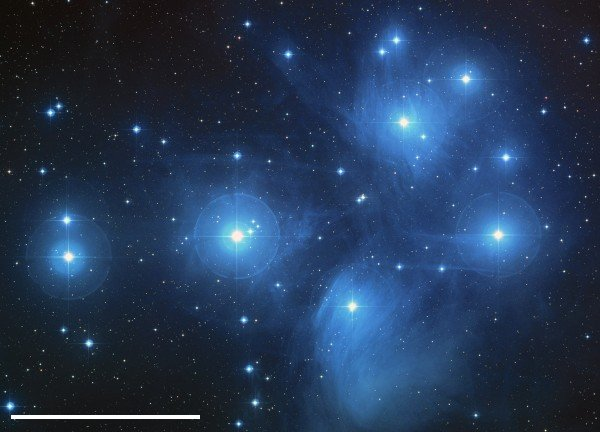
\includegraphics[width=\textwidth]{Figures/0_Pleiades_scale.jpg}
        \caption{The Pleiades, open cluster}
        \label{Fig:0_openglobular1.open}
    \end{subfigure}
    ~ 
    \begin{subfigure}[b]{0.4\textwidth}
        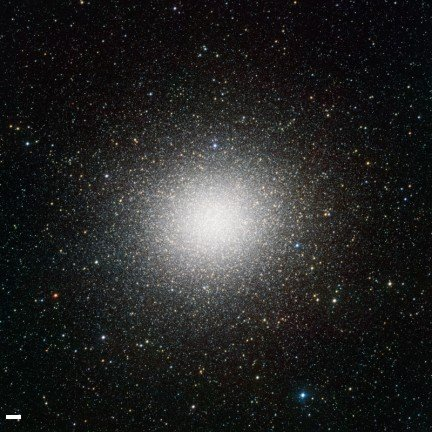
\includegraphics[width=\textwidth]{Figures/0_omega_centauri_scale.jpg}
        \caption{$\omega$ Centauri, globular cluster}
        \label{Fig:0_openglobular1.glob}
    \end{subfigure}
     \caption{Examples of various types of cluster. White bars at the lower left of each pictures show 1 parsec .The dust present in (a) scatters starlight producing this blue haze. (b) contains one million stars and is the largest known star cluster in the Milky Way.\\\textit{Credits: NASA, ESA, AURA/Caltech; ESO/INAF-VST/OmegaCAM}}
     \label{Fig:0_openglobular}
\end{figure}



As we will see, clusters are also crucial to understand stellar formation. They harbour the most massive and young stars, which cause large-scale ionisation, winds and shockwaves from their explosive death in supernovaes. Massive stars caused the re-iniozation of the entire known universe 400 Myr after the Big Bang. To understand massive stars is to understand star formation, and to understand star formation is to understand star clusters.



%
%\begin{figure}
%\center
%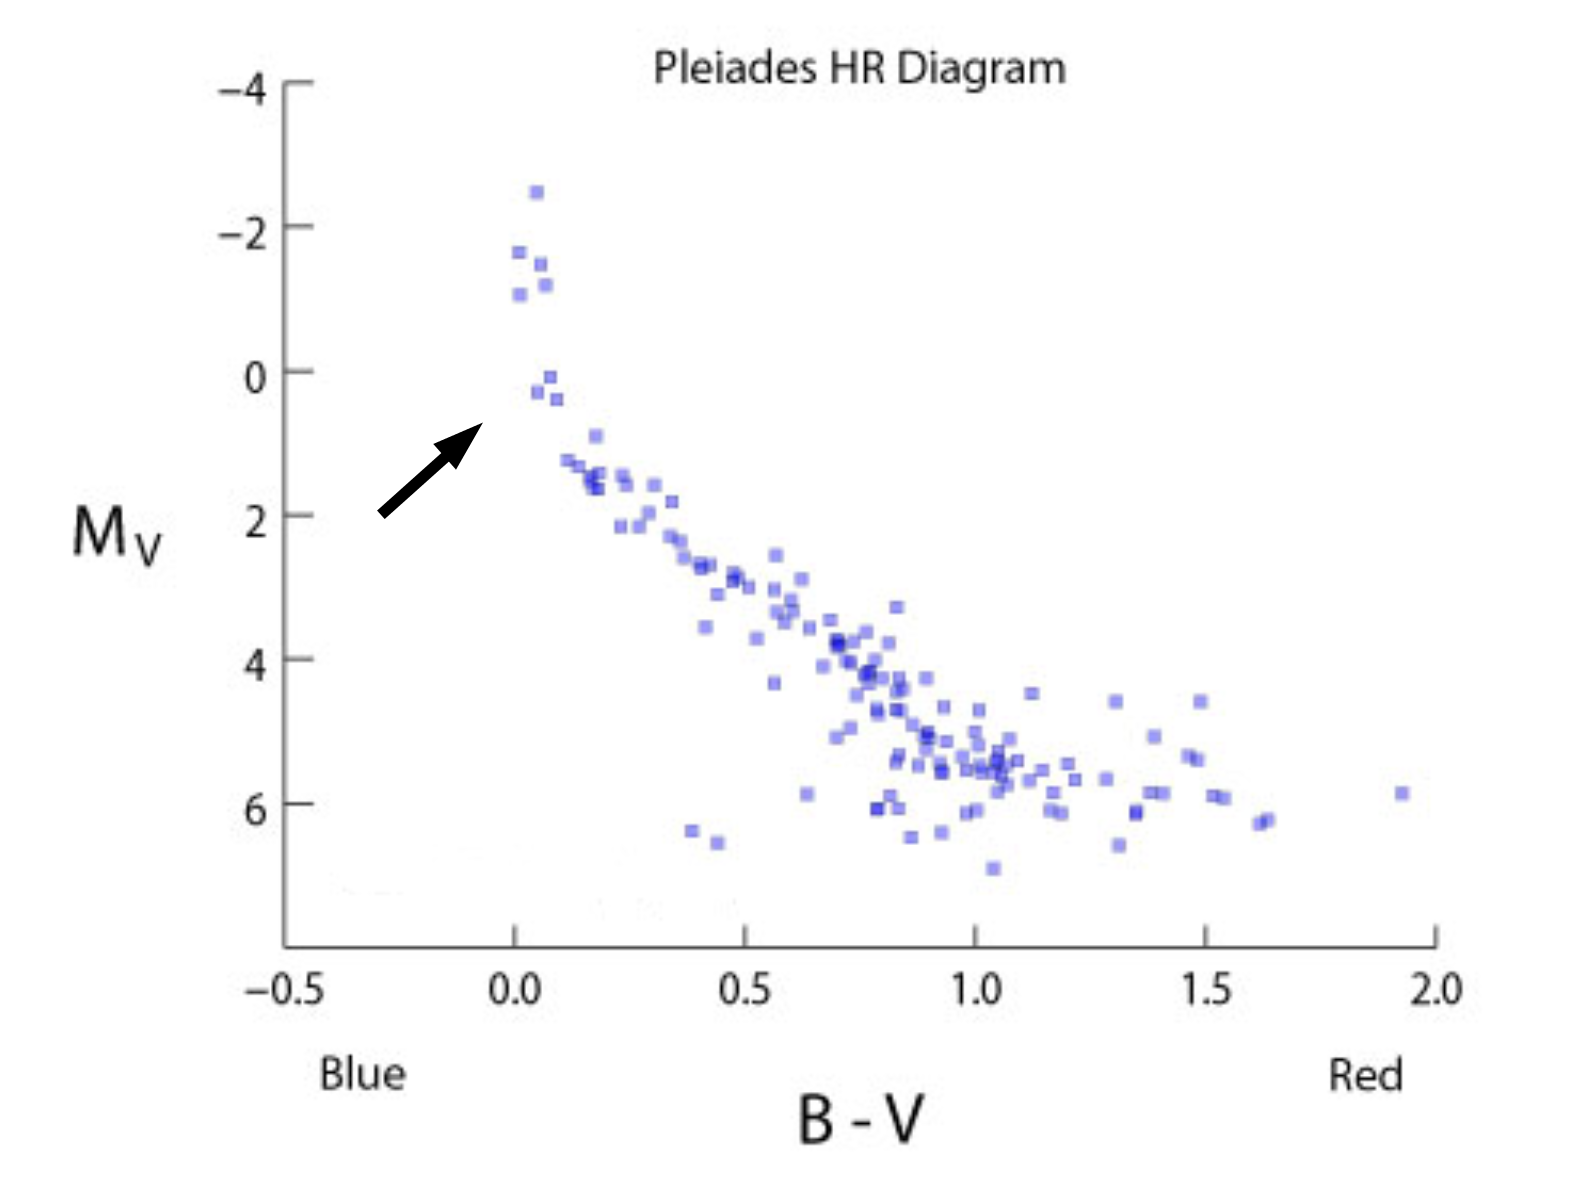
\includegraphics[width=0.45\linewidth]{Figures/0_HRDiagram_Pleiades.png}
%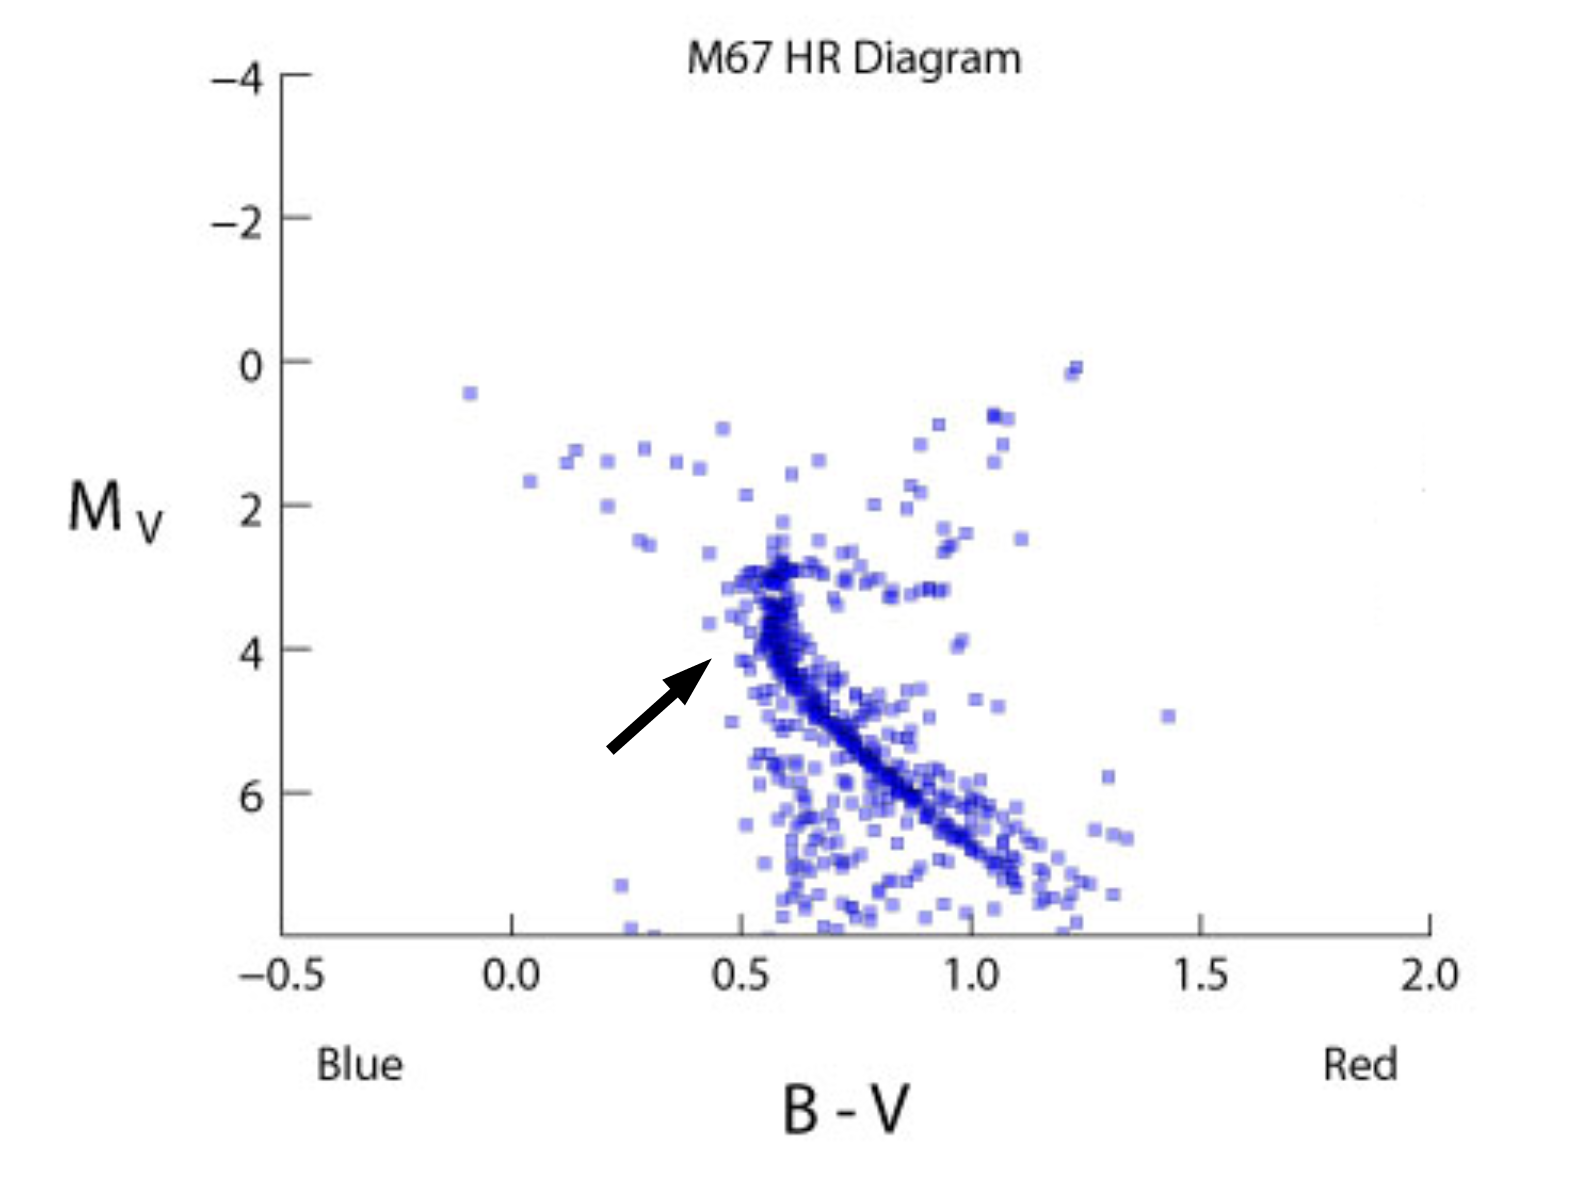
\includegraphics[width=0.45\linewidth]{Figures/0_HRDiagram_M67.png}
%\caption{Hertzprung-Russel diagram of the Pleiades and M67. An arrow points at the Main-Sequence turn-off for each cluster. The figures were taken from the \href{http://www.astrophysicsspectator.com/topics/stars/HertzsprungRussellClusters.html}{Astrophysics Spectator} website and data can be found in \protect\cite{Stassun2002,Kharchenko2004}  }
%\label{Fig:0_HR}
%\end{figure}
%
%One example is the ability to date a cluster, thus its members, through the main-sequence turn off. On figure~\ref{Fig:0_HR} is shown the Hertzprung-Russel diagram for two different clusters: The Pleiades and M67. The HR diagram shows the luminosity of the star versus its color, redder on the right, bluer on the left. Stars spend most of their life on the Main Sequence, with the most massive, luminous blue stars on the left, and red fainter smaller stars on the right. Massive stars have shorter lives and depart from the main sequence before small stars. Looking at the Main Sequence turn-off in the HR diagram of a cluster tells us the mass of the stars currently leaving the MS, which gives its age and that of all other stars. As seen on the figure, the Pleiades are younger (100Myr) than M67 ($\sim$ 4 Gyr) as the stars leaving the MS are more massive.

\subsection{Types of star clusters}

Star clusters are historically divided into two main categories: globular clusters and open clusters. As observationnal techniques improved, categories tended to blend into a spectrum of size, age, and dynamical state, with Young Massive Clusters, embedded clusters and OB associations. Several of these categories have significant overlap, but each one emphasizes a particular characteristic of star cluster, thus these are useful for a comprehensive discussion.


\begin{figure}
	 \begin{subfigure}[b]{0.415\textwidth}
        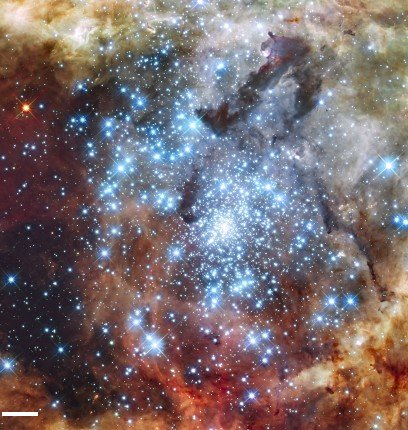
\includegraphics[width=\textwidth]{Figures/0_R136_scale.jpg}
        \caption{R136, Young Massive Cluster}
        \label{Fig:0_openglobular2.ymc}
    \end{subfigure}
    ~ 
    \begin{subfigure}[b]{0.55\textwidth}
        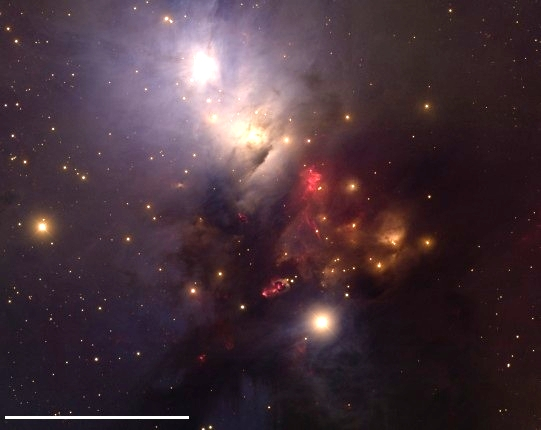
\includegraphics[width=\textwidth]{Figures/0_NGC1333_scale_contrast.jpg}
        \caption{NGC 1333, embedded cluster}
        \label{Fig:0_openglobular2.emb}
    \end{subfigure}
    
    \caption{Examples of various types of cluster. White bars still show 1pc. (a) is  surrounded by its primordial nebula while (b) is still inside it, the picture is a composite of visible and infra-red light. \textit{Credits: NASA, ESA, F. Paresce;T. Rector(U.Alaska Anchorage), H. Schweiker}}
    \label{Fig:0_ymcemb}
\end{figure}

\begin{itemize}


\item[\textbf{Globular clusters}] are old and massive stellar systems. Most of them are older than 10 Gyr and more massive than $10^4~M_\odot$. The most massive known Globular cluster in the Milky Way is $\omega$ Centauri, with $4~10^6~\Mo$ \citep{Dsouza2013}, see ref~\ref{Fig:0_openglobular1.glob}. They only contain stars, without any dust or gas. The 150 known globular clusters in the Milky way are scattered in the disk and the halo, with a higher concentration near the bulge \citep{Harris1996}. 

\item[\textbf{Open Clusters}] are lighter objects, rarely more massive than $10^3 \Mo$. They are also younger, with ages ranging from a few Myr to a few Gyr \citep{Dias2002}. In fact, open clusters do not have a clear definition other than the implicit and historical characteristic of "not being a globular cluster" and have a very wide range of characeteristics. Overall, they are faint, sometimes irregular and volatile objects. Their small mass and lower density make them vulnerable to tidal disruption from passing massive clouds on nearby orbits. The pleiades are a famous example,see ref~\ref{Fig:0_openglobular1.open}

\item[\textbf{OB associations}] contain even less stars than open clusters, a few dozens in average. They get their name from the very massive luminous O and B type stars they contain, sometimes more massive than 50 $\Mo$. Such stars do not survive more than a few million years, OB association are thus young objects located in active star forming regions. They are often found near other associations, in a hierarchical structure.  Their density is much lower than a typical cluster, about $0.1 ~\Mo \textrm{pc}^{-3}$ \citep{Wright2014},  in fact most are unbound and dissolving objects. See \cite{Garcia2010} for a detailed census and description of the OB associations in IC 1613.

\begin{figure}
\center
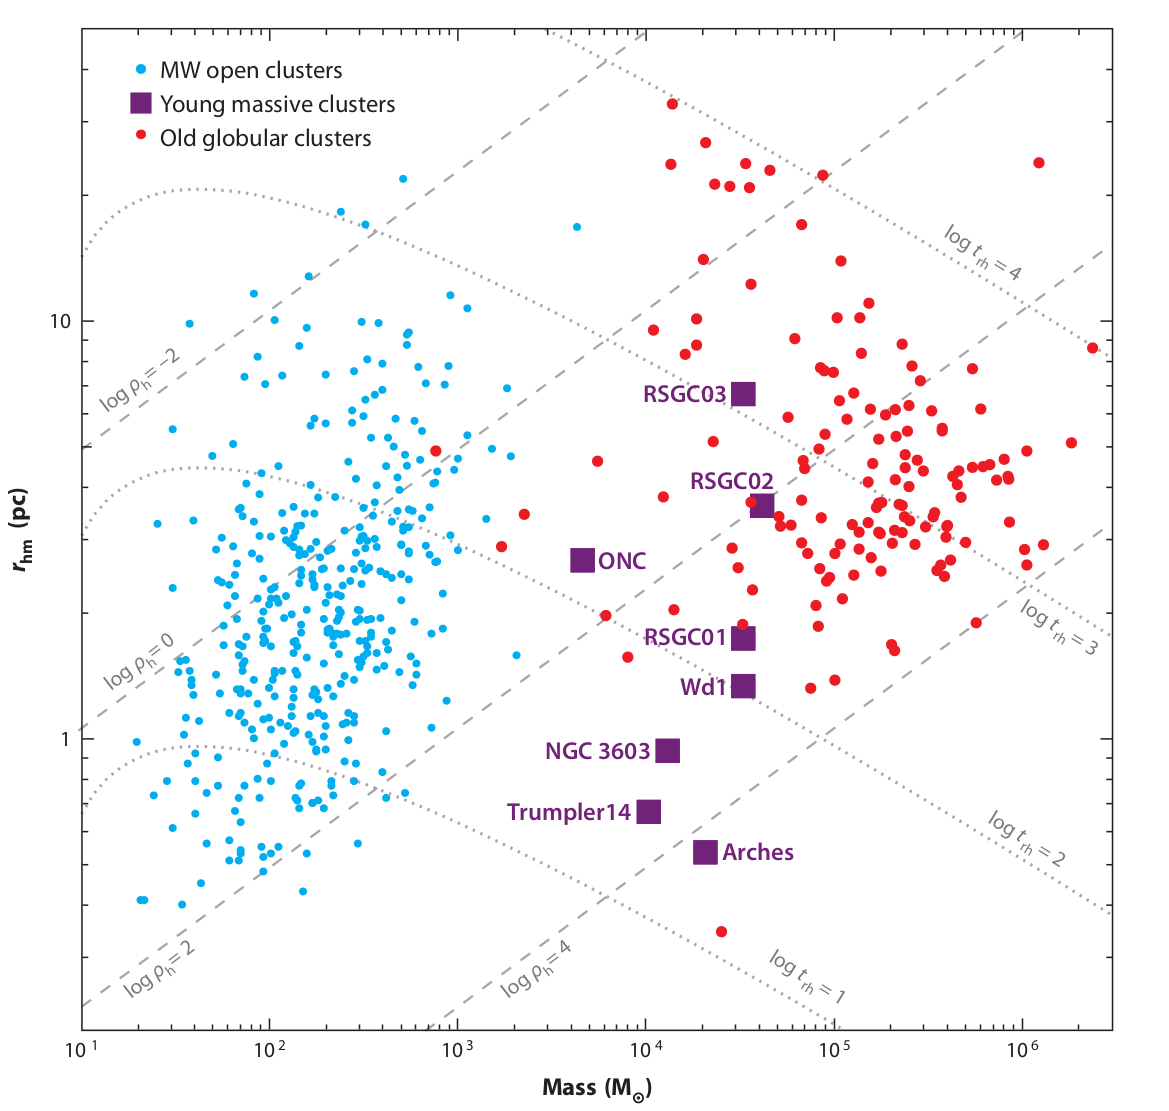
\includegraphics[width=0.65\linewidth]{Figures/0_MassRadiusClusters.png}
\caption{Radius-Mass Diagram for Milky Way clusters. Blue dots are open clusters, red dots Globular clusters and purple squares show Young Massive Clusters. Dashed lines show constant density within half-mass radius $\rho_h = 3M/8\pi r^3_{hm}$ and dotted lines show constant relaxation time. The plot was taken from the review \protect\cite{PortegiesZwart2010}.}
\label{Fig:0_SPZ}
\end{figure}

\item[\textbf{Embedded clusters}] are the youngest star clusters in the sky. Most of the stars, protostars and cores are still inside their primordial cloud, dust obscuring their optical light. The development of infrared astronomy unveiled the internal structure of these objects. As the gas is fully evacuated by 10Myr \citep{Lada2003}, embedded clusters are younger and observed to be substructured \citep{Kuhn2015}. Some have ongoing star formation, like NGC 1333, a very young embedded cluster with both proto-stars and stars, see \cite{Foster2015} and Fig~\ref{Fig:0_openglobular2.emb}.

\item[\textbf{Young Massive Clusters}], or YMCs, are considered to be globular cluster progenitors. The review by \cite{PortegiesZwart2010} provides a definition of YMCs: bound systems more massive than $10^4 \Mo$ and younger than 100 Myr. Only a handful of such systems are known in the milky way (see Fig~\ref{Fig:0_SPZ}). The most studied YMC of the galactic neighborhood is R136, with a mass $\sim 10^5 \Mo$ \citep{Andersen2009}, see Fig~\ref{Fig:0_openglobular2.emb}. It is located in the Tarentula nebula, the most active known star forming region in the local group, inside in the Large Magellanic Cloud \footnote{A dwarf irregular galaxy orbiting the milky way.}. YMCs are found in large number in intense star forming environment such as starburst galaxies and galaxy mergers like the Antenna galaxies \citep{Whitmore2010}.

\end{itemize}





"All stars form in clusters" is a recurring statement in the field of stellar and cluster formation. Near Infra-Red (NIR) studies of star forming region yielded an star formation rate from embedded clusters of $\sim 3~10^3~\Mo ~\textrm{Myr}^{-1}~ \textrm{kpc}^2$ \citep{Lada2003} while the same estimation for field stars in the milky way gives $\sim3-7~10^3~\Mo~\textrm{Myr}^{-1}~\textrm{kpc}^2$ \citep{Miller1979}. Another clue at the clustered nature of star formation is that high-mass O stars are for the vast majority, clustered, see \cite{DeWit2005}. Due to their short life, O stars are often observed at the very location of their birth, or not very far. However, some work by, e.g,  \cite{Gutermuth2011} seemed to point at a spatially hierarchical star formation. So stars do form in clusters, as in, in groups, but these groups are diverse and their dynamical evolution is complex.






%Due to their age, GCs are dynamically evolved. Introducing the relaxation time, defined in \cite{BT} by:
%\begin{equation}
%\label{Eq:0_relaxation}
%t_{relax} = 0.1 \frac{N}{logN} t_{cross} = 0.1 \frac{N}{logN} \frac{R_{hm}}{\sigma}
%\end{equation}
%
%with $t_{cross}$ the crossing time, defining the time a star takes to cross the system and $\sigma$ the internal velocity dispersion. The relaxation time is the time it takes for a system to erase its initial condition, perturbation per perturbation. GCs have a relaxation time of about a Gyr, they are relaxed systems. Various models have been put forward for the structure of GCs, the King \citep{King1966} and Plummer \citep{Plummer1911} models are the most widely used.


%\item NGC 2808 is reported to contain 1.4 $10^6~\Mo$ \citep{Boyles2011}. 
%
%Globular clusters had long been thought to have an homogeneous stellar population. Yet, a study by \cite{Piotto2007} showed NGC 2808 contained at least three different stellar sequences. Many other GCs has been shown to contain multiple populations. As this cannot be explained by the natural age spread arising from a continuous star formation at the birth clusters, such observations have far-reaching implication on their formation scenario. Several hypothesis are being explored, such as GCs being the outcome of mergers \citep{Pasquato2016} or a sequence of distinct star forming events \citep{Dantona2016}, with no consensus for now.


%\begin{itemize}
%
%\item 47 Tucanae (NGC 104) is one of the most massive known globular cluster in the Milky Way. It is estimated to contain about 1.5.$10^6~\Mo$ and to be 13 Gyr old\citep{Forbes2010}. Its core is extremely dense, as many GCs, with a central density up to $10^6 \Mo/\textrm{pc}^3$. Such a concentration of stars is a favorable environment for stellar collisions, which create what is called \textit{stellar exoticae}, stellar object not following the standard evolutionnary path, such as blue stragglers. Blue stragglers are stars too luminous and too massive compared to the age of the cluster, likely formed out of colliding stars. 47 Tuc exhibits a population of such objects, as well as others: Cataclysmic variables, X-ray binaries, etc. These are the direct consequence of the very dense environment of globular clusters such as 47 Tuc.
%
%\item Messier 12 (NGC 6218) is on the light end of the mass spectrum with 9.$10^4~\Mo$ \citep{Marks2010}. Such a low mass is however thought to be due to the cluster's dynamical history. Globular clusters have orbits around the galaxy, some more dangerous than others. For example Palomar 5 is currently disappearing after violent encounters with the galactic center. A study by \cite{DeMarchi2006} showed M12's orbit probably also passes close to the galactic center. Subjected to the strong tidal forces of the galactic bulge, M12 would have lost about 4/5 of its original mass. This scenario is backed by the mass function of M12. The mass function is the distribution of stellar masses, and its slope is thought to be more or less universal, though it appears unusually flat in M12. The tidal shock would have preferentially depleted low mass stars, as a process known as mass segregation tends to have massive stars sink at the center and low-mass stars overpopulate the outskirts of the system. 
%
%\item NGC 2808 is reported to contain 1.4 $10^6~\Mo$ \citep{Boyles2011}. NGC 2808, as all others GCs, had long been thought to have an homogeneous stellar population. Yet, a study by \cite{Piotto2007} showed NGC 2808 contained at least three different stellar sequences. As this cannot be explained by the natural age spread arising from a continuous star formation at the birth of the cluster, such observations have far-reaching implication on its formation scenario, and those of many GCs with multiple populations. Several hypothesis are being explored, such as GCs being the outcome of mergers \citep{Pasquato2016} or a sequence of distinct star forming events \citep{Dantona2016}, with no consensus for now.
%
%\end{itemize}

%
%\begin{figure}
%\label{Fig:0_GlobularClusters}
%\center
%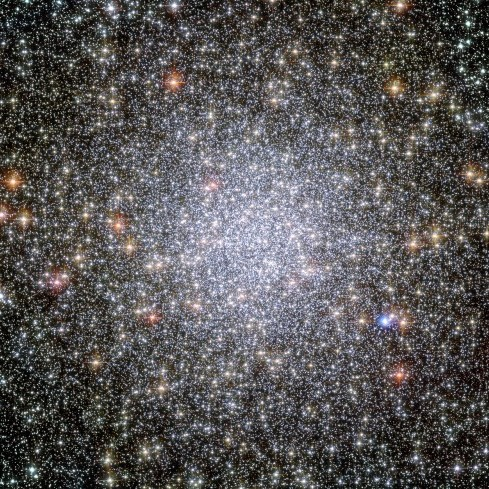
\includegraphics[width=0.3\linewidth]{Figures/0_47Tuc.jpg}
%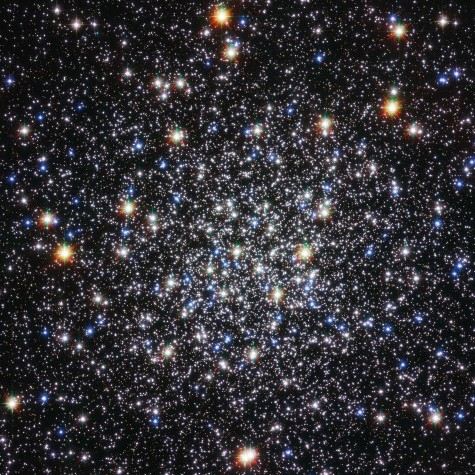
\includegraphics[width=0.3\linewidth]{Figures/0_M12.jpg}
%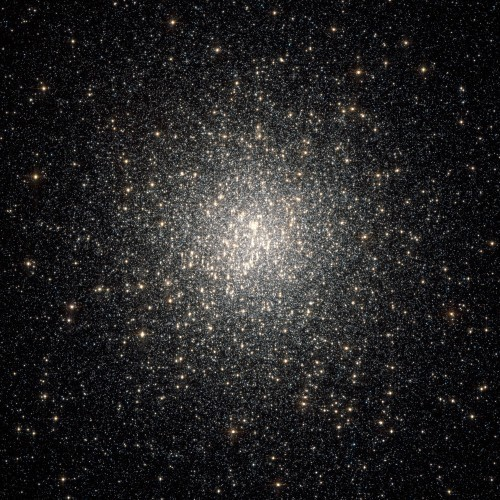
\includegraphics[width=0.3\linewidth]{Figures/0_NGC2808.jpg}
%\caption{From left to right: 47 Tucanae, Messier 12 and NGC 2808. Credits: ESA/Hubble. }
%\end{figure} 


\section{Some important dynamical concepts}


\subsection{Virial theorem}

A self-gravitating system is a system bound by its own gravity. This applies to a star, a molecular cloud, a star cluster or a galaxy. In all cases, gravity is set against a counteracting force that prevents the total collapse of matter into a single point. This force can be pressure for stars and clouds, but for stellar systems such as clusters and galaxies, it is the agitation of its components, the kinetic energy of the stars. Other forces include magnetic pressure or tidal fields.

The exchange between the gravitational potential energy and the kinetic energy follows the famous virial theorem, written in the general form \citep{McKee2007,BT}:

\begin{equation}
\frac{1}{2} \frac{d^2 I}{dt^2} = 2 ( E_k - E_{k,s}) +  E_p + E_{tides} + E_m
\end{equation}
with $I$ the moment of inertia, $E_k$ the kinetic energy, $E_p$ the potential energy. $E_{k,s}$  a thermal pressure surface term, $E_{tides}$ the energy injected by a tidal field and $E_m$ the magnetic pressure. For a stationnary system, $\frac{1}{2} \frac{d^2 I}{dt^2} = 0$, and in a purely gravitational system with N particles, there is no thermal or magnetic pressure. Finally, if we consider an isolated system,$E_{tides}=0$ and the virial theorem can be written in its more common form:

\begin{equation}
2 E_k + E_p = 0
\end{equation}

with :

\begin{equation}
 E_k = \sum_{i=1}^N m_i v_i^2 ~~~~\textrm{and}~~~~ E_p = - \sum_{i=1}^N \sum_{j>i}^N \frac{G m_i m_j}{\| \bold{r_i} - \bold{r_j}\| } .
\end{equation}

We define the virial parameter $Q$ as:
\begin{equation}
Q = - \frac{E_p}{E_k},
\end{equation}

$Q=0.5$ is a system in virial equilibrium. If the amplitude of the velocities is not sufficient to counteract the current value of potential energy, $Q<0.5$, the system is said to be dynamically cold, or \textit{subvirial}. While if the stars are too close together compared to the velocity amplitudes, $Q>0.5$, the system is hot and \textit{survirial}. If $Q>1$, the total energy is positive and the system is unbound. 


\subsection{Dynamical timescales}

Dynamical systems tend to virial equilibrium. In such self-gravitating systems, it is useful to define a few dynamical time scales. The most simple one is the \textbf{crossing time}, defined as:
\begin{equation}
\label{Eq:0_tcr}
t_{cr} = \frac{R}{\sigma}
\end{equation}
with $R$ the typical radius of the system and $\sigma$ the velocity dispersion. It is the typical time it takes for a particle to cross the system. Another crucial timescale in stellar dynamics is the \textbf{relaxation time}. \cite{BT} define it as:

\begin{equation}
\label{Eq:0_tr}
t_r \simeq \frac{0.1 N}{ln N} t_{cr}.
\end{equation}

In a self-gravitating system, stars have orbits. If N is large enough, the potential inside the system is smooth and stars have stationnary orbits. The relaxation time is the timescale at which the impact of numerous encounters a star endures is comparable to the motion of its initial orbit. In other words, the initial conditions of a system are dynamically erased by collisional evolution after a relaxation time.

In a relaxed cluster, the core is dense with a high velocity dispersion, whereas the outskirts, the halo, is less dense and stars are slower. The definition from equation (\ref{Eq:0_tcr}) and (\ref{Eq:0_tr}) imply the relaxation time changes with distance to the center. It is therefore useful to define a global timescale for the whole system, the \textbf{half-mass relaxation time} defined by \cite{Heggie2003}:


\begin{equation}
\label{Eq:0_trhm}
t_{rh} \simeq   \frac{0.138}{ln N} \sqrt{ \frac{N}{G m}} R_h^\frac{3}{2}
\end{equation}

with $m$ the mass of a star and $R_h$ the half-mass radius. Let us compute two examples, taking G in appropriate units:

\begin{equation}
G \simeq 4.48 \times 10^{-3}~~ \textrm{pc}^3 ~\textrm{Myr}^{-2} ~\Mo^{-1}.
\end{equation}

A cluster with 1000 stars of 0.5$\Mo$ and $R_{h} = 1$ pc has $t_{rh} = 13$ Myr, while a cluster with 10$^6$ stars of the same mass and a $R_{h} = 6$ pc have $t_{rh} = 3.1$ Gyr.


Equations (\ref{Eq:0_tr}) and (\ref{Eq:0_trhm}) assume identical stellar masses in the system. In a real cluster, stars have different masses, differently affected by collisional evolution. The most massive stars cause gravitational focusing and exchange energy with other stars at a higher rate. They lose their energy to lighter stars, progressively sinking at the center. \cite{Heggie2003} give an estimation of the segregation timescale $t_{seg}(m_1)$of a mass $m_1$:
\begin{equation}
t_{seg}(m_1) = \frac{m_1}{\langle m \rangle} t_{rh}
\end{equation} 
so a 30 $\Mo$ star in the previous 1000 star cluster will have a relaxation time of $\frac{0.5}{30} 13 = 0.21$ Myr = 210,000 years, much faster. A mass spread in a system speeds up considerably its collisional evolution.



\subsection{Static models}

It is useful to have a static reference model for a self-gravitating system at equilibrium. Considering a relaxed system with enough particles, one can use a statistical description to model its evolution, namely the "collisionless Boltzmann equation":

\begin{equation}
\frac{\partial f}{\partial t} + \bold{v} \cdot \nabla_r f - \nabla \Phi \cdot \nabla_v f = 0
\end{equation}

with $f(\bold{r},\bold{v},t)$ the phase space distribution and $\Phi$ the gravitational potential. There are several solutions to this equations, these are "static" models for star clusters as they are considered in equilibrium. Of course, the collisional equation can never be fully neglected and these models are approximations. We present here two models: Plummer and King. Both have a constant density in the center, the core, but they differ by their general behaviours. 

The \textbf{Plummer model} is a simple model with a null potential at infinity. It is defined by its potential as a function of radius \citep{BT}:

\begin{equation}
\Phi(r) = - \frac{G M}{\sqrt{r^2 + b^2}}
\end{equation}

with $b$ the Plummer parameter, setting the depth of the central potential and the core radius. From this expression, one can derive the radial density distribution:

\begin{equation}
\label{Eq:0_plummerrho}
\rho(r) = \frac{3 M}{4 \pi b^3} \left( 1 + \frac{r^2}{b^2} \right) ^{- \frac{5}{2}}
\end{equation}

Equation (\ref{Eq:0_plummerrho}) makes the computational generation of a cluster straightforward, which is why the Plummer model has been widely used in numerical simulations of star clusters.
However, a Plummer model theoretically extends to infinity, and is not consistent with many globular cluster observations. Another, more complex, model has the observers on his side. The \textbf{King model} has been sucessfully used to fit light-profiles of globular clusters \citep{King1981}. It is defined as a distribution in energy:

\begin{equation}
  f_k(E)=\begin{cases}
    f_0 \left(e^{-2j^2E} - e^{-2j^2E_0}\right)  , & \text{if $E<E_0$}.\\
    0, & \text{otherwise}.
  \end{cases}
\end{equation}

with j a free parameter. The core radius can be tuned through a parameter $W_0 =2j^2(E_0 - E_c)$ with $E_c$ the rest energy at the center. 

The main difference with the Plummer model can be seen in Fig~\ref{Fig:0_plummerking}: for a given core radius, King's density decreases slower than Plummer, but does falls to zero at a given radius contrary to Plummer that continues to infinity.

\begin{figure}
\center
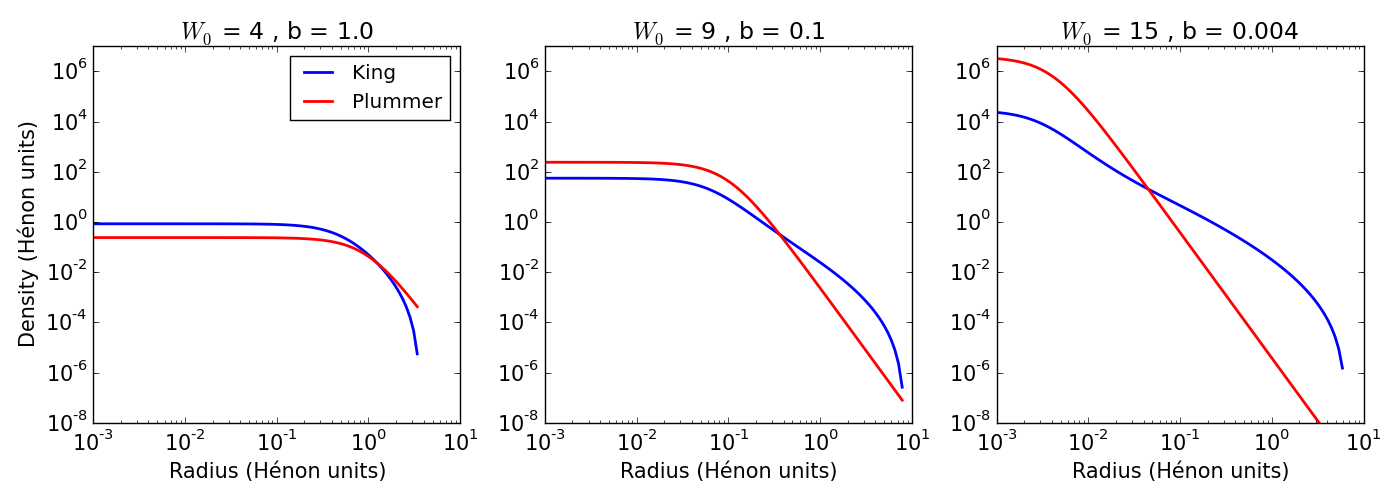
\includegraphics[width=0.95\linewidth]{Figures/0_kingplummer.png}
\caption{Comparison of King and Plummer models density as a function of radius, for similar core radiuses.}
\label{Fig:0_plummerking}
\end{figure}





\section{The origin of star clusters}

\subsection{From gas to stars}

The interstellar medium, or ISM, is made of dust and gas in various phases, densities and temperatures, ranging from a hot ionized medium ($T>10^5 K$ and $n < 0.01 cm^{-3}$) to a cold neutral medium ($T<100 K$ and $n > 10 cm^{-3}$),  see \cite{Field1969}. Finally, in colder denser regions, $T\sim 10k$ and $n>30cm^{-3}$, the hydrogen takes molecular form H$_2$ in what is called molecular clouds. The dust contained in these regions makes them optically thick, obscuring background stars. These "holes in the sky", as William Herschel exclaimed upon the Dark Ophiucus Nebula\citep{Houghton1942}, come in different sizes, from the "bock globules" to Giant Molecular Clouds (GMCs).
The interstellar dust absorbs the light in the visible and re-emits it in the infrared, thus the advent of infrared astronomy unveiled the interior of molecular clouds. In particular, recent observations with the Herschel Space Observatory showed a prevalence of filaments in clouds, see \cite{Andre2010}.

Star formation occurs in the higher density clumps or filaments inside the clouds. The origin of these overdensities has been the object of extensive theoretical development for 60 years. Turbulent motion was very early on designated as the main cause of overdensity. Turbulence is the transfer of energy from large scales to small scales, creating motions on small scales from a large energy driver. The well known Kolmogorov incompressible turbulence is hardly applicable to the ISM, as it is highly compressible \citep{Scalo1998}, instead, molecular clouds are subject to supersonic turbulence, or Burgers turbulence \citep{Frisch2001}. Nearby supernovas or tidal perturbation feed energy into the cloud, which is transfered through turbulence to smaller scales as supersonic internal motions, shocks forming overdense sheets. \cite{McKee2007} argue that filaments originate both from the intersection of such sheets and the primordial morphology of the cloud, as self-gravitating pressureless matter condense as filaments \citep{Springel2005}.

\begin{figure}
\center
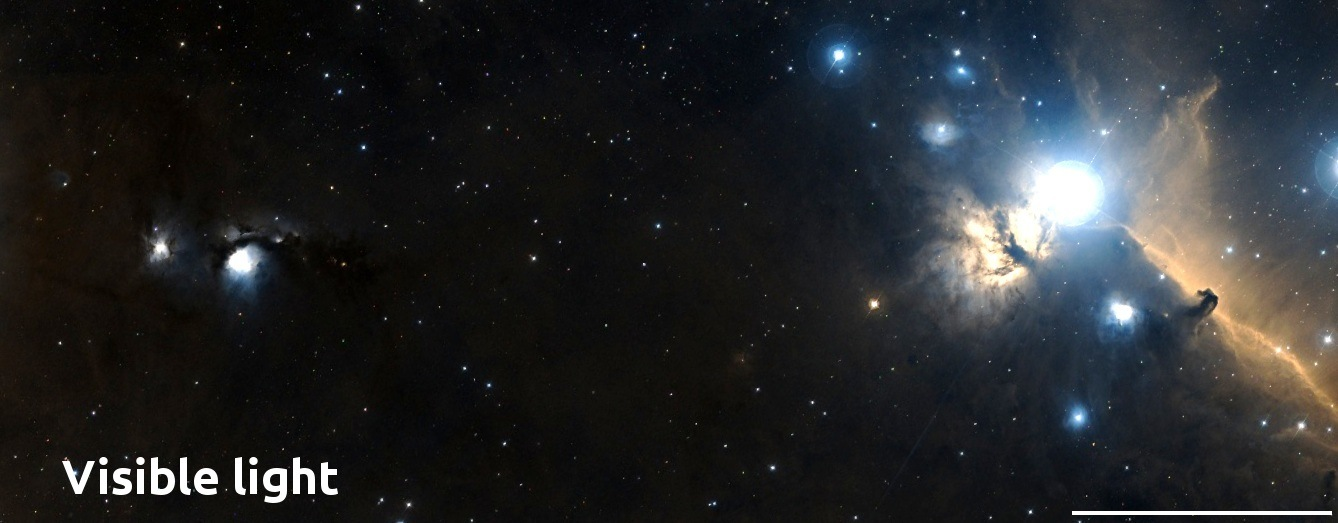
\includegraphics[width=0.95\linewidth]{Figures/0_horsehead_visible2}
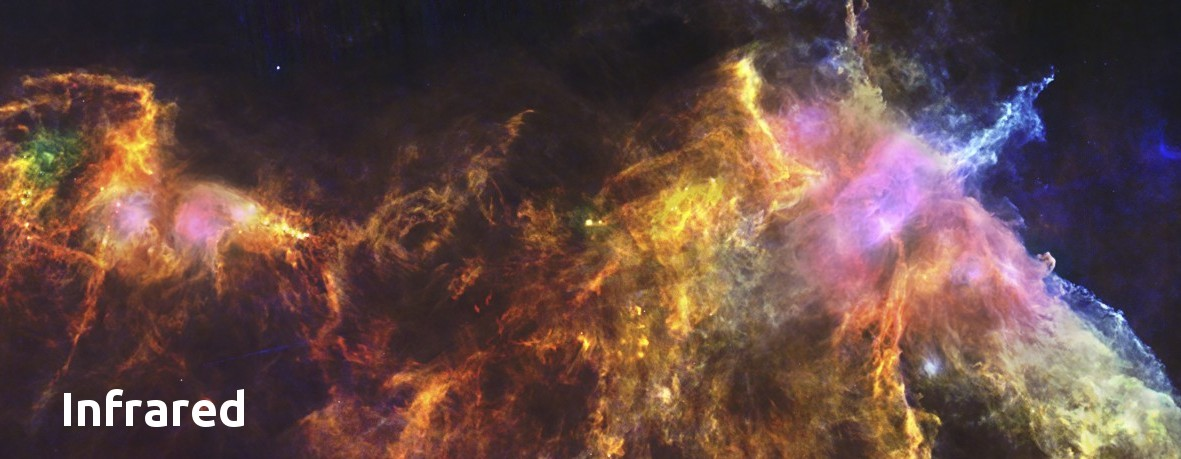
\includegraphics[width=0.95\linewidth]{Figures/0_horsehead_infrared}
\caption{Visible light  and infrared view of a part of the Orion star forming complex. Horshead nebula is visible on the right, as well as the very bright star Alnitak, part of the Orion belt. NGC 2071 and 2068 are visible on the left. Pink infrared coloring shows radiation from very bright yong massive stars forming in the cloud. Colder filaments are visible all around. White on lower right of visible shows 1 parsec. \textit{Credits: Digitized Sky Survey; ESA/Herschel/PACS}. }
\label{Fig:0_horsehead}
\end{figure}

Individual condensates of matter called cores form in clumps and filaments, these are stellar seeds (Fig~\ref{Fig:0_proto_1}). To collapse, they have to overcome their magnetic and thermal pressure and their internal turbulence. The idealized picture of an hydrodynamical collapse relies on an estimation of the Jeans length $\lambda_\textrm{J}$, the maximum wavelength of a density perturbation in a uniform gas above which pressure cannot respond fast enough and gravitational collapse is triggered. The corresponding Jeans mass M$_\textrm{J}$, of diameter $\lambda_\textrm{J}$ is the minimum mass of a cloud to collapse. These quantities are derived in \cite{BT} and are expressed

\begin{align}
\lambda_\textrm{J} & = \sqrt{\frac{\pi}{G \rho}} c_s \\
	 & \simeq  0.2 \textrm{pc} \left( \frac{c_s}{0.2 ~ \textrm{km.s}^{-1}} \right) \left( \frac{n}{10^3 ~ \textrm{cm}^3} \right)^{-\frac{1}{2}}
\end{align}

\begin{align}
M_\textrm{J} &=  \frac{4 \pi}{3} \rho ( \lambda_\textrm{J} )^3 =    \left( \frac{\pi}{6} \right) \frac{c_s^3}{G^\frac{3}{2}\rho^\frac{1}{2}} \\
 & \simeq  2.7 \Mo \left( \frac{c_s}{0.2 ~ \textrm{km.s}^{-1}} \right)^3 \left( \frac{n}{10^3 ~ \textrm{cm}^3} \right)^{-\frac{1}{2}}
\end{align}

with $c_s$, $\rho$ and $n$ the local sound speed, density and number density. These are the typical values expected for a prestellar core with such sound speeds and number densities. The molecular gas remains isothermal throughout the collapse, as the center radiates away the thermal energy from the increased density. When density reaches $10^10$ cm$^{-3}$, the dust mixed in the protostellar material turns the core of the cloud optically thick, energy cannot be radiated away anymore, temperature rises and collapse stops. It continues to accrete material, increasing its central density and temperature. When T reaches 2000K, molecular hydrogen starts to dissociate, absorbing energy. This allows a second collapse, stopped when all initial molecular hydrogen has been dissociated. The resulting core is called a protostar (Fig~\ref{Fig:0_proto_2}), its density profile is peaked in the cente and reaches about $10^{21}$ cm$^{-3}$ and a temperature of 20,000K. The protostar has a mass of $\sim$ a thousandth of its future stellar mass, as most of it is acquired during the next phase, accretion. Angular momentum from the original cloud shapes the gaseous envelope into a disk around the protostar, and magnetic activity starts creating jets (Fig~\ref{Fig:0_proto_3}). This stage has been divided into several classes, based on the Spectral Energy Distributions (SED) emitted by the objects, has the emission shifts from far infrared to mid, then near-infrared as the envelope is accreted. See \cite{Evans2009} for an historical description of the SED classes and \cite{Larson1969} for a theoretical overview of the principles of collapse and protostellar formation. 



\begin{figure}
    \centering
    \begin{subfigure}[b]{0.19\textwidth}
        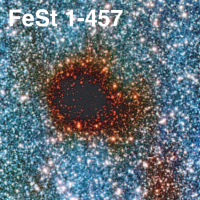
\includegraphics[width=\textwidth]{Figures/0_proto_1.jpg}
        \caption{  Starless core\\\centering (NIR)}
        \label{Fig:0_proto_1}
    \end{subfigure}
    \begin{subfigure}[b]{0.19\textwidth}
        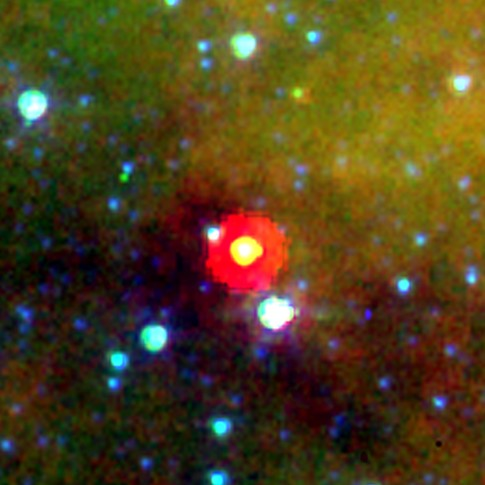
\includegraphics[width=\textwidth]{Figures/0_proto_2.jpg}
        \caption{Young protostar  \\ \centerline{ (IR)}}
        \label{Fig:0_proto_2}
    \end{subfigure}
        \begin{subfigure}[b]{0.19\textwidth}
        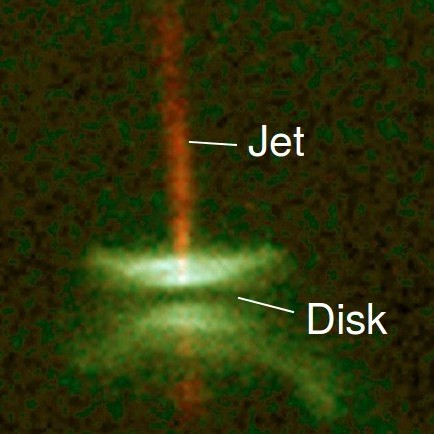
\includegraphics[width=\textwidth]{Figures/0_proto_3.jpg}
        \caption{Protostar \\\centering (IR,UV)}
        \label{Fig:0_proto_3}
    \end{subfigure}
        \begin{subfigure}[b]{0.19\textwidth}
        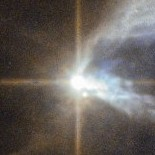
\includegraphics[width=\textwidth]{Figures/0_proto_4.jpg}
        \caption{Pre-MS star \\ \centering (visible)}
        \label{Fig:0_proto_4}
    \end{subfigure}  
        \begin{subfigure}[b]{0.19\textwidth}
        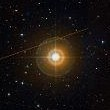
\includegraphics[width=\textwidth]{Figures/0_proto_5.jpg}
        \caption{MS star \\\centering (visible) }
        \label{Fig:0_proto_5}
    \end{subfigure}
     \caption{Stages of stellar birth. (a) is just cold molecular gas and contains no central source yet. (b) is more advanced, though hidden in visible light, its central protostar shines in infrared.The protostar in (c) is actively accreting its disk and produces jets. (d) is a pre main-sequence star, free from its envelope and surrounded by primordial gas. (e) is the mature stellar stage: the main sequence.\textit{Credits: \protect\cite{Kandori2005}; NASA/JPL-Caltech/Evans,N; Burrows,C/HST-NASA; ESA/Hubble \& NASA; DSS}}
     \label{Fig:0_protoevolution}
\end{figure}





After about a Myr, accretion stops and the object becomes a Pre-Main Sequence (PMS) star (Fig~\ref{Fig:0_proto_4}). It slowly contracts, following the Hayashi track, first described by \cite{Hayashi1961}. The source of energy of the star is still gravitational contracting, until central temperature reaches 10$^6$K and hydrogen starts fusing into Helium. The  object enters the Main Sequence and begin its life as a proper star(Fig~\ref{Fig:0_proto_5}).


\subsection{Substructure and early dynamical evolution}

Observations show molecular clouds are substructured (see e.g. \citealt{Cambresy1999}). This substructure can be seen as a fractal distribution \citep{Elmegreen1996} or a network of filaments \citep{Andre2010}, both consistent with compressible turbulence \citep{McKee2007}	. This hierarchical structure is inherited by the cores and protostars that emerges from the overdensities, as many observational studies of star forming regions shows \citep{Schneider1979,Hartmann2002,Bressert2010}. Examples of substructured young clusters include the Taurus Ariga region, $\rho$-Ophiucus and Aquila, details and other examples can be found in both volumes of \textit{The handbook of star forming region} \cite{Reipurth2008}.  

However, other young clusters do not display such fractal, clumpy or filamentary structure. Instead, they are smooth, centrally condensed systems. The most known example is the Orion Nebula Cluster, or ONC. Located in the heart of the Orion complex, the largest and most active star forming region in the solar neighborhood, the age of the ONC is estimated to a few Myr. \cite{Hillenbrand1998} found no clumps or filaments in the stellar distribution of the cluster, but a smooth distribution with a high density core formed by the Trapezium, a dense system of massive stars. This mass segregation, if not fully primordial, implies that some amount of dynamical evolution took place in the ONC since the formation of the stars. This dynamical evolution could have erased the initial substructures.

These observations point at a rough picture of substructured stellar formation and early evolution: when the newly born stars emerges in clumps, if the background tidal field is weak and the star forming region sits well inside its Roche radius, the clumps then progressively merge and converge to the system barycentre to form a unique, relaxed  self-bound association over a  course of a few crossing time. This picture is backed up to some extent by hydrodynamical simulations of fragmentation modes in the turbulent ISM \citep{Klessen2000,Bate2003,MacLow2004,Offner2009,Maschberger2010} and by recent observationnal clues that subclusters show dynamical traces of mergers \citep{Kuhn2015b}. 

\begin{figure}
\center
    \centering
    \begin{subfigure}[b]{0.48\textwidth}
        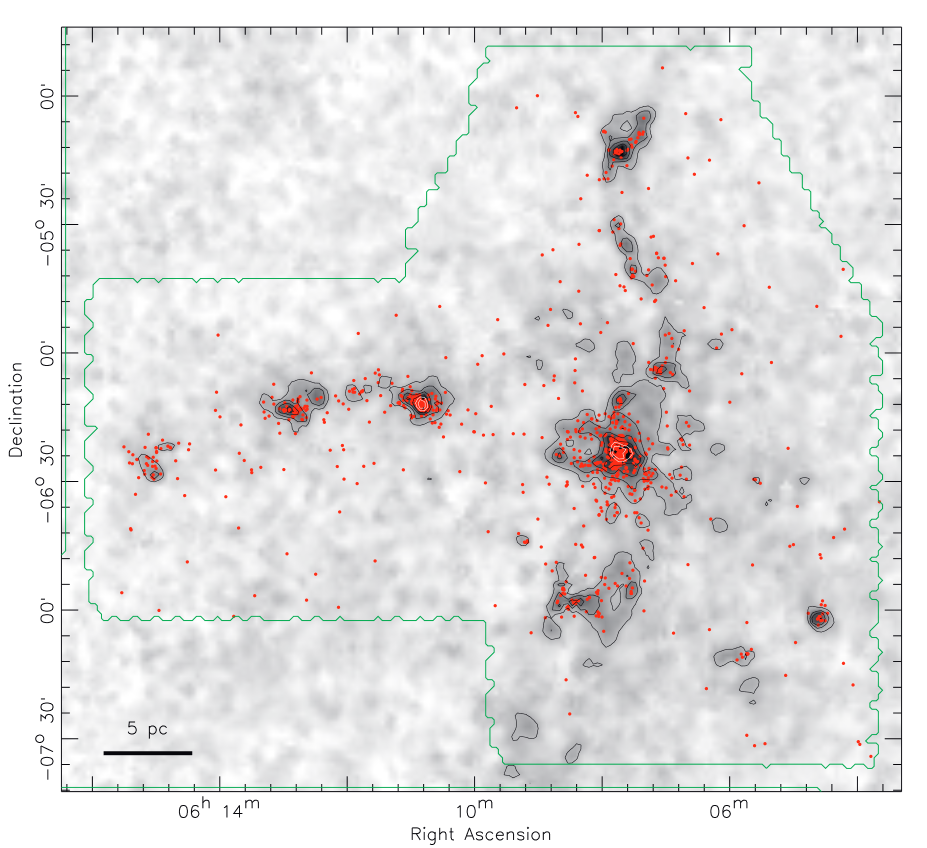
\includegraphics[width=\textwidth]{Figures/0_clumpsobserved.png}
        \caption{Observed distribution of gas and protostars}
        \label{Fig:0_clumps_obs}
    \end{subfigure}
    \begin{subfigure}[b]{0.48\textwidth}

        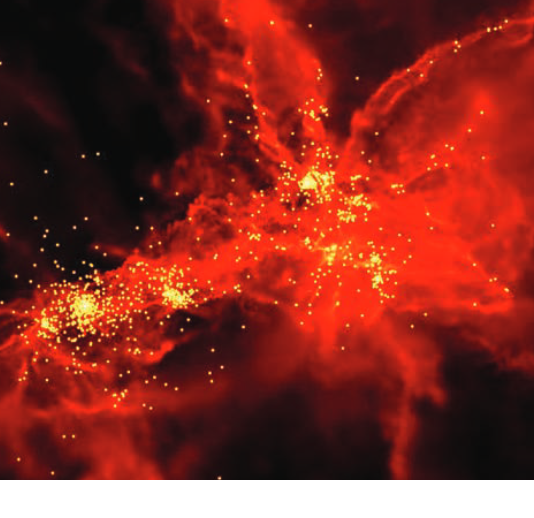
\includegraphics[width=0.9\textwidth]{Figures/0_clumpssimulated.png}
        \caption{Hydrodynamical simulation}
        \label{Fig:0_clumps_sim}
    \end{subfigure}
\caption{(a): observational data from the Monoceros R2 star forming region. Protostars are shown as red  points and gas density (traced through extinction) is shown in greyscale. The figure was extracted from \cite{Gutermuth2011}. (b): hydrodynamical simulation of a star forming region yellow points are star-like sink particles and red levels show gas density. The figure was extracted from \cite{Bonnell2011}.}
\label{Fig:0_clumps}
\end{figure}

Figure \ref{Fig:0_clumps} shows the similarity of stellar distribution obtained by observations and simulations of star forming regions.


\subsection{Star formation efficiency and infant mortality}

In their seminal paper on embedded clusters, \cite{Lada2003} coined the term "infant mortality" for young star clusters. Comparing the populations of embedded clusters and older open clusters, the authors concluded clusters had a 90\% mortality rate before 10~Myr. This is explained by the traditionnal picture of gas expulsion in clusters: a portion of the gas in a molecular clouds form a group of protostars, which quickly accrete their envelope, then start nuclear burning. This portion is expressed as the star formation efficiency:
\begin{equation}
\epsilon = \frac{M_*}{M_* + M_{gas}}
\end{equation} 
with $M_{gas}$ the remaining gas after star formation. This gas is thought to be ejected from the young cluster through photo-ionization (the UV radiation from massive stars ionize the neutral gas which heats up and expands), jets and outflows (young stars ejecting matter during accretion), winds (ejection of matter from stars surfaces at high speeds), and supernovae (shockwave from the explosive death of a massive star). The gas expulsion occurs on a dynamical time, see \cite{Goodwin1997}. Considering a young cluster in dynamical equilibrium, the loss of the mass of the gas on such a short timescale can unbound the system, as the stars velocities are now too high for the new potential well. The young cluster then dissolves following the gas expulsion.
This picture is backed up by observations of young dissolving clusters \citep{Bastian2006} consistent with corresponding numerical models \citep{Goodwin2006}. Extensive analytical and numerical work have explored this process, e.g. \cite{Tutukov1978,Boily2003a,Boily2003b}, with an estimated minimum star formation efficiency of 30\% to remain bound after gas expulsion.

However, the picture is more complicated than it seems. First, the efficiency of stellar feedback is a complex problem, winds, photionisation and supernovaes have various impacts depending on the size and morphology of the clouds; they also seem to influence each other, for an overview of the problem see the serie of papers from \cite{Dale2011,Dale2013} and references therein. Furthermore, recent hydrodynamical simulations such as \cite{Pelupessy2012} show the exact timescale of gas removal has a crucial importance on the fate of the cluster, with a slow removal allowing survival with $\epsilon$ as low as 5\%.

\begin{figure}
\center
    \centering
    \begin{subfigure}[b]{0.48\textwidth}
        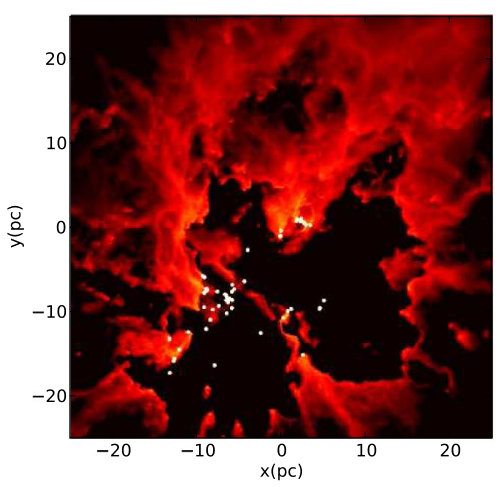
\includegraphics[width=0.9\textwidth]{Figures/0_ejectionwind.png}
        \caption{Simulation of gas expulsion}
        \label{Fig:0_ejection_1}
    \end{subfigure}
    \begin{subfigure}[b]{0.48\textwidth}

        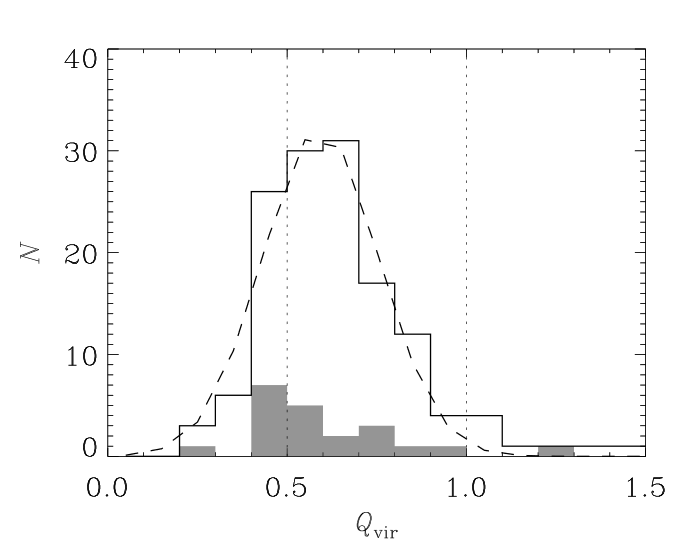
\includegraphics[width=\textwidth]{Figures/0_virializedclumps.png}
        \caption{Virial states of stellar clumps}
        \label{Fig:0_ejection_2}
    \end{subfigure}
\caption{(a): hydrodynamical simulation of wind-induced gas expulsion around a small cluster, the figure was extracted from \cite{Dale2013}. (b) virial parameter of stellar clumps in a star forming hydrodynamical simulation, ignoring the potential of the gas to predict their post-expulsion fate. The figure was extracted from \cite{Kruijssen2012}.}
\label{Fig:0_clumps}
\end{figure}


Finally, most of the previously mentionned simulations assumed a relaxed embedded stellar system. However, as mentionned in previous section, star formation is substructured. Dynamical evolution between clumps and subclusters occurs on timescales comparable to gas expulsion, making the stellar spatial distribution of huge importance for survival, as shown by \cite{Farias2015}. Hydrodynamical simulations (e.g \citealt{Kruijssen2012}) even point at subclusters being primordially quasi gas-less due to localized high $\epsilon$, thus increasing the importance of substructure over gas expulsion.


\section{Simulating star clusters evolution}


\subsection{Hydrodynamical simulations}

I invoked hydrodynamical simulations multiple times in the previous section. Let us look at them in more details. To model the formation of a star cluster from a core-less molecular cloud is no easy task. The model has to reproduce turbulence, core condensation, gravitational collapse, accretion, and for the most realistic ones, radiative cooling and stellar feedback. Two numerical path has been explored in the past: AMR and SPH.

Adaptative Mesh Refinement, AMR, is an Eulerian approach. The hydrodynamical equations (conservation of mass, momentum, the equation of state) are discretized and solved on a grid of cells following the finite volumes methods (see the RAMSES code, \citealt{Teyssier2002}). Smoothed Particle Hydrodynamics, SPH, is a Lagrangian approach: instead of looking at inputs and outputs of matter in a cell, the gas is subdivided in particles free to move in the system. They are attributed a density, temperature and pressure. This method is akin the N-body integrator, and many SPH codes can work as purely gravitational integrators. SPH is popular in star formation simulations, as the problem is itself Lagrangian: grains of highly dense matter condensates and move around. Even if these codes can handle high density contrast, the collapse and formation of a protostar can still bring the numerical computation to a standstill. The usual workaround is the use of sink-particles: passed a given density threshold, several particles are merged into a single point-like object able to accrete any infalling matter. This works well though it suppresses any physical process below this accretion limit, usually a few to a hundred AU. \citep{Bate1997}.

The precision, size and complexity of large scale cluster formation simulations have been steadily improving for 20 years (see \citealt{Turner1995,Klessen2000,Bate2003,Offner2009,Myers2014} and citations). Nevertheless, no simulation to date include realistic cooling processes, radiative and wind feedback, magnetic fields and dust chemistry, all at the same time. All these are crucial to achieve precise and realistic simulation of the star formation process. Moreover, one of the most detailed star formation simulations to date, e.g \cite{Bate2012}, only form a few hundred stars and evolved them for less than 0.2~Myr with a simulation run time of several months.

However, good results are already being achieved, see the short review by \cite{Clarke2012}. Stellar properties and general structure agree with observations and interesting results are being obtained. \cite{Maschberger2011} and \cite{Moeckel2011} have noted that massive stars tend to sit at the heart of gas clumps in hydrodynamical simulations, some as the result of merger events with low-mass proto-stars. 

In a nutshell, hydrodynamical simulations are not yet fully realistic, but they provide a good approximation of reality for small clusters and allow exploration or early dynamical processes.


\subsection{Artificial substructure}

There is a persitent difficulty to bridge over self-consistently from the star formation phase, to the equilibrium configuration of bound clusters. Hydrodynamical calculations of star forming regions evolve for  up to a few $\times 10^5$ years, when a stable configuration would require several $\times 10^6$ years at typical cluster densities of $10^4$ to $10^5$ stars per cubic parsec. A way to overcome this issue is to switch to purely gravitational N-body simulations once the stars formed and most of the gas has been either accreted or expulsed. It is computationaly less expensive and allows for longer integration of larger systems.

It is then essential to obtain a good model of the stars phase-space distribution at the end of a hydrodynamical simulation. While King and Plummer model have a known distribution one can sample from, no such thing exist for the clumps and filamentary structure of the newborn stellar objects in a star-forming regions. Several methods have been explored to solve this.



\begin{figure}
\center
    \centering
    \begin{subfigure}[b]{0.48\textwidth}
        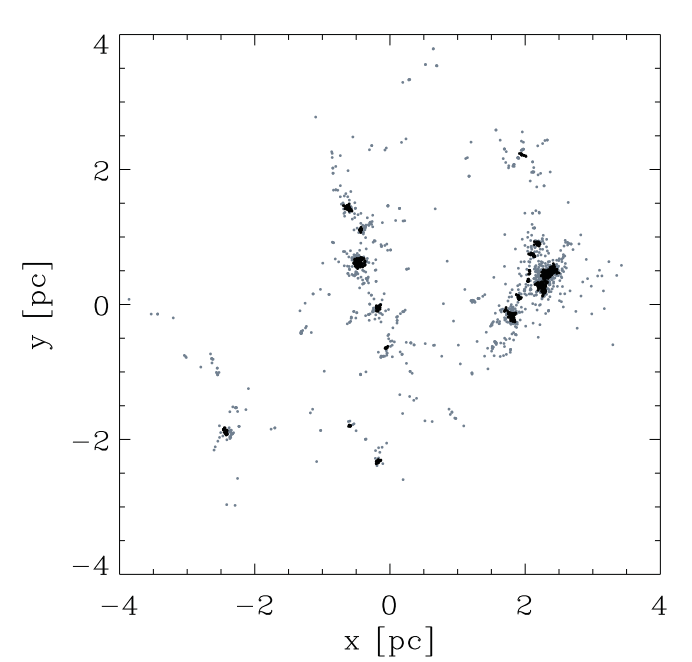
\includegraphics[width=\textwidth]{Figures/0_bonnell.png}
        \caption{Hydrodynamical output}
        \label{Fig:0_substructure_0}
    \end{subfigure}
    ~~
    \begin{subfigure}[b]{0.48\textwidth}
        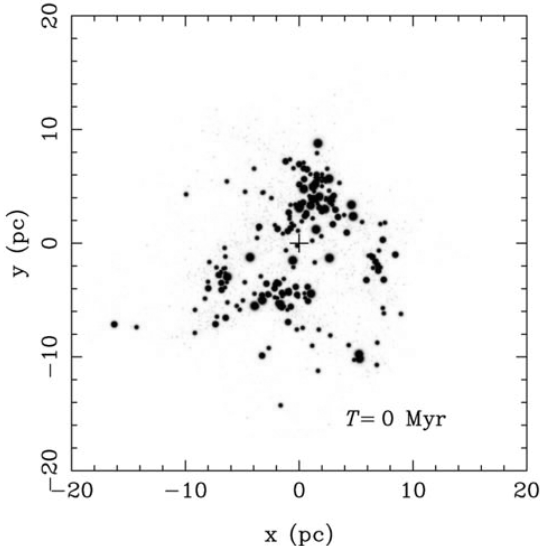
\includegraphics[width=0.93\textwidth]{Figures/0_fujii.png}
        \caption{Stellar spawning}
        \label{Fig:0_substructure_1}
    \end{subfigure}
    \\
    \begin{subfigure}[b]{0.48\textwidth}
        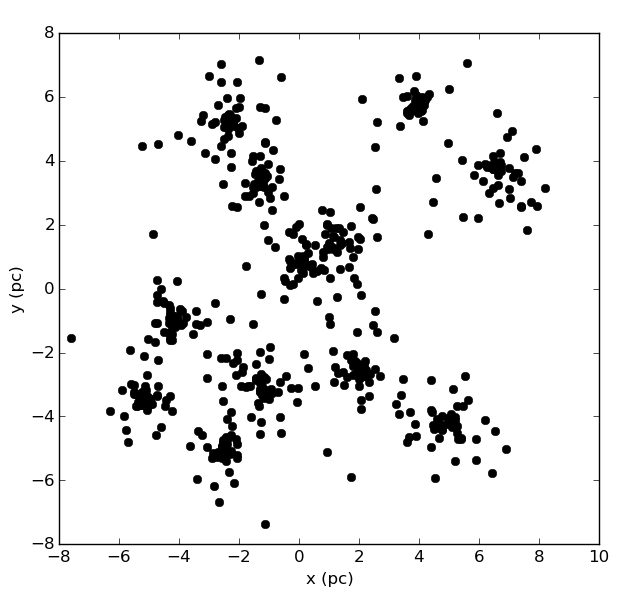
\includegraphics[width=0.95\textwidth]{Figures/0_plummers.png}
        \caption{Multiple Plummer}
        \label{Fig:0_substructure_2}
    \end{subfigure}
    \begin{subfigure}[b]{0.48\textwidth}
        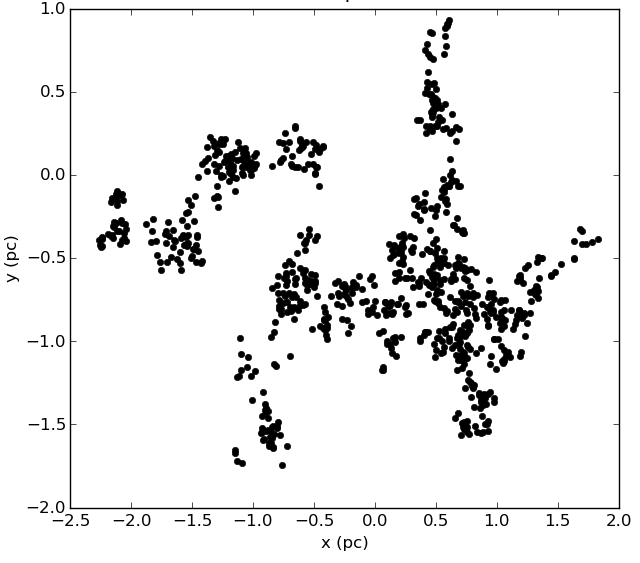
\includegraphics[width=\textwidth]{Figures/0_fractals.png}
        \caption{Fractal configuration}
        \label{Fig:0_substructure_3}
    \end{subfigure}
\caption{Representation of four methods to generate substructures. (a) is extracted from \citep{Kruijssen2012}, constructed with data from \cite{Bonnell2003}, (b) is extracted from \cite{Fujii2015}. (c) and (d) were generated for this work.}
\label{Fig:0_substructures}
\end{figure}

 
\begin{itemize}
\item[\textbf{Sink particle distribution}] is the most straightforward solution. \cite{Moeckel2010} took the distribution of sink particles formed in the hydrodynamical simulation by \cite{Bate2009} and directly converted it as a stellar distribution, preserving the masses, positions and velocities of the "stellar seeds". This is probably the best initial conditions for nbody simulations of young clusters that can be achieved, at the cost of speed, sampling and size. The initial hydrodynamical simulation took months to complete, making it hard to run it again and impossible to run it multiple times to obtain a good statistical sampling of the model. The size of the cluster achieved cannot exceeds 1000 stars given the current state of hydrodynamical simulations.

\item[\textbf{Stellar spawning from hydrodynamics}] is a variant of the previous method. \cite{Fujii2016} started from hydrodynamical simulations of massive molecular clouds and stopped the integration once the main structures had formed but before local gravitational collapse had set in. Stars were then spawned in space following the distribution of gas. This enables larger clusters and quicker initial conditions of structures. However, the velocity distribution of these new stars is artificial, as it can at best inherit the gas velocity, without including the impact of the early collisional evolution that occurs between protostars in the clumps.

\item[\textbf{Scattered Plummer spheres}] is an analytic answer to the substructure problem. \cite{McMillan2007} created a clumpy model for a young star cluster by spawning several Plummer spheres randomly in space. This is almost immediate and is a good approximation. The authors obtained interesting results on the inheritance of mass segregation during mergers. However, clumps within a young star clusters have no reason to follow a Plummer profile, this places a constraint on the clumps internal dynamics which bias the dynamical evolution.

\item[\textbf{Fractal models}] were introduced by \cite{Goodwin2004} and has been used in numerous studies ever since, e.g. \cite{Allison2009b,Kouwenhoven2010,Parker2016}. The idea is to grow a 3D pseudo-fractal tree with probabilistic branching, down to a given level, turning the final leaves into stars. The method is fast and the result is spatially realistic, fitting the observation that finds a fractal structure in the molecular clouds and star forming regions. However, the velocity distribution is artificial, drawn from successive gaussians at each levels. The clumps will relax when integration starts, shaking the whole system right off the bat.

\end{itemize}

It seems the generation of substructure has to balance realism and compututational cost. The most realistic method is too costly, and most of the quicker alternatives are disconnected from the dynamical effect arising from the collisional effects young stars undergo inside a clumpy configuration.



\section{Binary stars}

\subsection{What is a binary star ?}

When two massive bodies of mass $m_1$ and $m_2$ interact gravitationally, they can have different types of trajectory depending on their total energy:

\begin{equation}
E = E_k + E_p = \frac{1}{2} m_1 v_1^2 + \frac{1}{2} m_2 v_2^2  - \frac{G m_1 m_2}{\| \bold{r_1} - \bold{r_2}\| }.
\end{equation}

%\begin{itemize}
%\item[$\bold{E>0}$], the system is unbound, the bodies follow hyperbolic trajectories. They have a distance of closer approach then move away from each other forever.
%\item[$\bold{E=0}$], the system is marginally unbound, the bodies follow parabolic trajectories.
%\item[$\bold{E<0}$], the system is bound, the bodies have stable elliptical orbits around each others.
%\end{itemize}

If $E<0$, they are bound and locked in a binary system. Such systems are characterised by their semi-major axis $a$, their eccentricity $e$, their period $p$, their total mass $m_t = m_1 + m_2$, mass ratio $q = m_2/m_1$ with $m_1$ being the primary, more massive than $m_2$.
Mass, period and semi-major axis are related by Kepler's third law:

\begin{equation}
\frac{G m_t}{4\pi^2} =  \frac{a^3}{p^2}.
\end{equation}

Interestingly, expressed in AU, $\Mo$ and years, $G \simeq 4 \pi^2$, thus the law can be written:

\begin{equation}
\left( \frac{m_t}{1 \Mo} \right) = \left( \frac{p}{1 \textrm{yr}} \right) \left( \frac{a}{1 \textrm{AU}} \right)^3 .
\end{equation}


The total energy of the binary can be expressed as a function of $a$ and $m_t$:

\begin{equation}
E = - \frac{G m_1 m_2}{2a} 
\end{equation}

\subsection{Why binaries ?}

Binary stars are extremely important for a variety of reasons. They can be a reservoir of energy, supporting the core of a cluster against collapse by giving away their internal energy to perturbers, effectively ejecting stars and heating the system, affecting its global evolution and stopping core collapse (e.g \citealt{Heggie1992}).

The properties of binary stars in dense stellar associations in particular may shed light on the discovery of multiple star-formation episodes in rich stellar clusters \citep{anderson2009}. For instance, binary stars enhance strong dynamical interactions which in turn may speed-up evolution off the main sequence and so boost enrichment of the ISM through winds (e.g., \citealt{Tailo2015}). Tight binaries of short-lived massive stars may evolve to produce exotic stellar remnants including black hole progenitors \citep{bacon1996,davies2009}. 

Finally, accurate knowledge of binary population in stellar clusters enable good estimation of their dynamical mass, as the integrated velocity dispersion is largely biased by the binaries internal motions, see \cite{Rubenstein1997}.

\subsection{Multiplicity fraction}

In a stellar population, some fraction of stars will be found in multiple systems: some  in binaries and some in higher order hierarchies. A hierarchical triple is a stable 3-body bound system, a binary of which one of the component is a binary itself. The same principle applies to quadruple, quintuple, etc. One of the brightest stars in the night sky, Castor, is a sextuple hierarchical system, with 6 stars in a stable system.

Counting binaries and multiples is not straightforward: do you count triples as two binaries or three stars in a multiple system ? In their SPH simulation paper, \cite{Goodwin2004a} discuss several ways to measure the degree of multiplicity among stars in a system, each of them quantifying different properties, such as companion probability, companion frequency or pairing factor. 

Let  S be the number of single stars, and B,T, and Q the number of binary-, triple-, and quadruple systems, respectively. The fraction of multiple stars bound in binaries, triples, .. to the total number of multiple plus single stars, is

\begin{equation}
\label{Eq:0_fm} 
f_m = \frac{B + T + Q}{S + B + T + Q}. 
\end{equation}

This last  measure is used in seminal observationnal papers \citep{DM91,Raghavan2010} and is our adopted choice. As pointed out by \cite{Hubber2005}, $f_m$ in Eq. (\ref{Eq:0_fm}) has several advantages: 1) it  may be  restricted to a given mass $m$, setting  $S_m$ the number of single stars, and $B_m,\, T_m,\, Q_m$  the multiple stars with a primary of that mass ;  2)  the multiplicity fraction is observationally robust: when a binary is being reclassified as a triple, or an even higher order multiple system, the fraction does not change. 
 These definitions may be extended to cover a mass range  in a coherent way, by substituting $m \rightarrow \langle m\rangle$, the mean value over the range. This is useful mostly when comparing  systems with different stellar mass functions. 


\subsection{Observed population}

The first real complete survey of binary solar-type stars in the field was performed by \cite{DM91}. This seminal paper was updated and completed by \cite{Raghavan2010}, who essentially confirmed the main results from the first study. They observed hundreds of F and G main-sequence stars in pairs and derived their binary parameters. The total binary fraction for these stars was found to be $\sim$ 53\% as binaries are quite common in any stellar population.
  The authors also derived a period distribution, extending from less than a day to more than a Myr. The distribution was consistently well fitted by a log-normal distribution. The period distribution for F and G stars (as well as K and M stars, see \citealt{Fischer1992}) is:
\begin{equation}
f( \log{P})\propto \exp \left[ \frac{- ( \log{P} - \mu_{logP})}{ 2 \sigma_{logP}^2} \right]
\end{equation}

with the peak value $\mu_{logP} = 5.03$, about 300 years, and the dispersion $\sigma_{logP} = 	2.28$, the distribution is shown on fig [TODO].

\cite{Raghavan2010} also compiled several observational studies of binaries with primaries of various spectral types. High mass stars, types O,B,A, (from 30+ down to 2$\Mo$) have a high multiplicity fraction, about 75\%  while lower mass stars such as M-dwarfs only have 10-30\% multiplicity. This trend of increasing multiplicity with increasing primary mass is found in many surveys.
Binary surveys are easier in the field due to the very large sample and low stellar density. To perform similar studies in young star clusters is much harder due to source crowding and embedded stars. \cite{Kouwenhoven2007} attempted to characterize the birth binary population in the OB association Scorpius OB2. They found a very high multiplicity fraction, consistent with 100\%, and a period distribution more consistent with a powerlaw than a log-normal distribution. From this survey and others, it is likely that the binary population in clusters undergoes an erosion through dynamical processing, with the field distribution as an end-result.

\subsection{Simulate binary populations in clusters}

As noted earlier, young clusters are born substructured, then undergo dynamical evolution. The rapid, global  merging of sub-structures would bring together stars at a different stage of their  formation (as in NGC1333, see \citealt{Foster2015}) while at the same time induce a shift from a clumpy Taurus-like profile to a more regular one. A simple but important question is how the internal dynamics of such complex configurations may affect the  characteristics of a population of binary stars. 

Many authors have explored this question through optimised initial conditions \citep{Kroupa2001,Marks2012} or fractal configurations evolved with N-body integrators \citep{goodwin2004,Allison2009,Parker2011,Parker2014}. A common feature to all these studies is that the binary fraction drops over time regardless of their components (masses), due e.g. to close star-star encounters or heating from the external galactic tidal field. \cite{Parker2014} pointed out that the distribution of semi-major axes $a$ of the field population is a strong function of the primary's mass: at fixed $a$, low-mass binaries carry less binding energy so the distribution cuts off at shorter separation ($\sim 20 $ AU) compared to that for binaries with a more massive primary ($\sim 300$ AU). Their study of fractal initial conditions show that gravitational dynamics enhances the dissolution of low-mass systems. This then provides a clue to account for the larger relative fraction of heavy stars in binaries, such as seen in a compilation by \cite{Raghavan2010}. 
 
  We note that hydrodynamical calculations of star formation have found young heavy stars to be preferentially found in dense clumps \citep{Maschberger2010}. Furthermore, it is not clear yet whether binary populations should be tailored according to the total system mass because of the limited range of $M \sim 10^2$ to $ \sim 10^3 M_\odot$ of these studies \citep{Kroupa2001,Parker2011,Parker2014}. Recall that the intensity of the tidal field is a prime agent of binary heating.  A trend with mass may be expected on the ground that the drive to equilibrium of more massive systems leads to deeper potential wells (e.g. \citealt{Aarseth1988,Boily2002}). A steep potential will give rise to strong tidal fields which may disrupt bound sub-systems \citep{Boily2004,Renaud2011}. A definitive assesment of this effect is difficult to reach because the results are a strong function of the system initial mass distribution and kinetic energy content \citep{Boily2002,Caputo2014}.




\newpage
\section{NBODY6}


NBODY6 is the second youngest iteration of the NBODY family, a suite of n-body integrators created by Sverre Aarseth. It can compute the gravitational interaction between up to 128,000 stars in a collisional fashion, meaning there is no softening of the potential, at any scale. This allows for very close binaries to form and remain in the system. To achieve its impressive performances, NBODY6 relies on several optimization technique which have been first developed in the 1960s and 1970s, and improved ever since. Here will be developped five major features of NBODY6, in chronological order of their implementation: H\'enon units, block time-step, KS-regularization, Hermite scheme and Ahmad-Cohen neighbour scheme. A full description can be found in Sverre Aarseth's book \citep{Aarseth2003}. Inspiration for this section should be credited to the user manual of NBODY6++, written by Emil Khalisi and Rainer Spurzem.

\subsection{H\'enon units}

NBODY6 uses a set of units specifically invented for the Nbody gravitational problem, the Nbody units, or H\'enon units (as prescribed by Douglas Heggie during the MODEST 2014 meeting). These units are based on three relations:

\begin{align}
G &= 1\\
M_t &= 1\\
E &= -\frac{1}{4}
\end{align}

With $G$ the gravitational constant, $M_t$ the total mass of the system and $E$ total energy of the system. For a virialized system, that is a relaxed system in which the virial ratio 
\begin{equation}
Q = - \frac{E_k}{E_p} = 0.5
\end{equation}
it comes that $E_k=0.25$ and $E_p = -0.5$ and, considering the definition of the virial radius 
\begin{equation}
R_v = - \frac{G M_t^2}{2 E_p} = 1.
\end{equation} 

This unit system was designed for virialized systems, but can be used for out of equilibrium systems, as long as they are bound ($Q <1$), with energy expressions functions of $Q$
\begin{align}
E_p  &= - \frac{1}{4(1-Q)}\\
E_k &= \frac{Q}{4(1-Q)}
\end{align}
which still fulfills the $E = -\frac{1}{4}$ condition. In practice, the H\'enon mass, radius and velocities are obtained through

\begin{align}
m_h &= \frac{m}{M_t}\\
r_h &= 4 (1-Q) |E_p| \cdot r\\
v_h &= \sqrt{ \frac{Q}{4(1-Q) E_k} } \cdot v
\end{align}

which can be used as an input for NBODY6.
\subsection{Block time-step}
 
In the first Nbody simulations, the system was integrated with an universal time-step, determined by the most accelerated star. A star in the outer regions of the cluster with a small velocity did not need to be updated that often. One of the first improvement  was the introduction of individual time-step: each star is attributed its own time-step, depending on the force that is applied to it and its derivative:

\begin{equation}
\label{Eq:0_timestep}
\Delta t_i =  \eta \sqrt{\frac{ |\bold{F_i}||\bold{F^{(2)}_i}| + |\bold{F^{(1)}_i}|^2 }{|\bold{F^{(1)}_i}||\bold{F^{(3)}_i}| + |\bold{F^{(2)}_i}|^2}}
\end{equation}
 
With $\bold{F}^{(j)}_i$ begin the j-th derivative of the force applied to particle i and $\eta$ a user-defined accuracy parameter. Such a complex formulation is the result of extensive tests and is quite robust for many special cases. Individual time-steps leads to desynchronized particles, hence the need to interpolate the positions of other particles to compute $\bold{F}_i$, which was achieved through fourth-order polynoms.
 
 To limit the amount of desynchronization, block-time steps were introduced. Instead of having as many time steps as particles, one only allows quantized power of 2 of an initial time step. $\Delta t_0$,$\frac{\Delta t_0}{2}$, $\frac{\Delta t_0}{4}$, $\frac{\Delta t_0}{2^i}$. All time steps are then commensurate and regularly fall back on the same time steps, minimizing the amount of interpolation during the force calculations.
 
\begin{figure}
\label{Fig:blocktimesteps}
\center
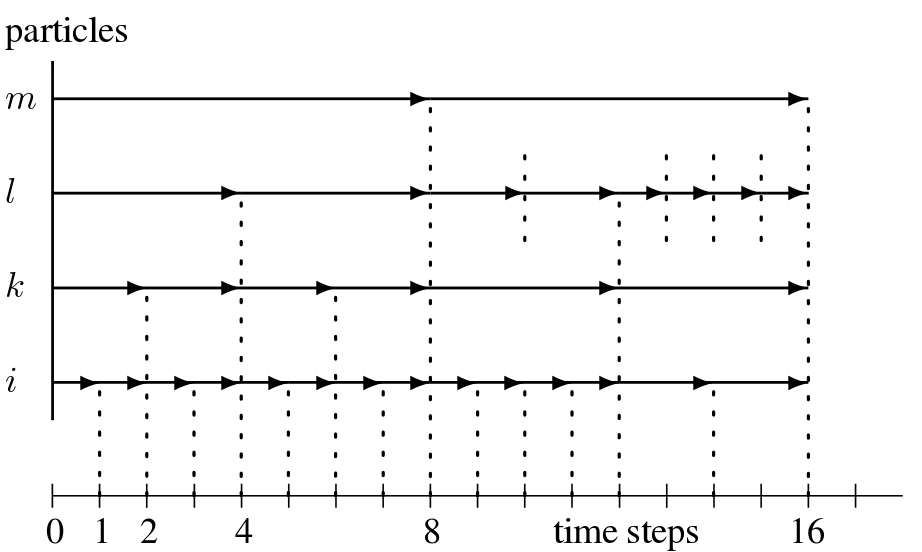
\includegraphics[width=0.6\linewidth]{Figures/0_block_timesteps.png}
\caption{Illustration of block time steps on 4 particles. Particles get their positions updated for each arrow symbol, common time steps are shown as vertical dotted lines. Figure from NB6++ User Manual. }
\end{figure} 
 
 
\subsection{KS-regularization}

Close binaries are extremely problematic in N-body simulations. They require a small time step as both binary components are much more accelerated than any other stars in the system, while the rest of the system is unaffected. Block time-step mitigate this problem, but the binary system still requires a lot of integration for an orbit that is essentially already known. Regularization is an answer to this problem. The essence of regularization is to decouple the integration of a sufficiently isolated sub-system, changing its coordinates to make integration easier, and including perturbations from external bodies. Several regularization scheme exist, NBODY6 implemented the Kustaanheimo-Stiefel method, or KS \citep{KS1965}.

Two bodies are candidates for regularization when their impact parameter is lower that the one needed for an orthogonal deviation, wherein their trajectory are deviated of 90$^\circ$:
\begin{equation}
b_\perp = 2G \frac{m_1 +m_2}{v^2_\infty}
\end{equation}
with $m_i$ components masses and $v_\infty$ relative velocity before encounter. This impact parameter can be converted to a time step computed through equation ~\ref{Eq:0_timestep}:
\begin{equation}
dt_{min} = \kappa \frac{\eta}{0.03} \left( \frac{r^3_{min}}{\langle m \rangle}\right)^\frac{1}{2}.
\end{equation}

To be actually regularized, two bodies have to have a mutual time step lower than $dt_{min}$ and fulfill two conditions:

\begin{align}
\bold{R_r} \cdot \bold{V_r} &> 0.1 \sqrt{ G(m_1+m_2)R_r}\\
\label{Eq:0_KSperturbation}
\frac{\left| \Delta \bold{F_r} \right| \cdot R^2_r}{G(m_1+m_2)} &< 0.25.
\end{align}

$\bold{R_r}$ and $\bold{V_r}$ being the relative velocities and positions of the particles and $\left| \Delta \bold{F_r} \right|$ the differential force applied to them, or perturbation. These conditions mean the subsystem is dynamically decoupled from external influence, but not unperturbed. When they are satisfied, the subsystem is regularized: it is replaced by the center of mass in the global system, and computed separately, with a set of changed coordinates. These coordinates are tailored for binary motion and close approach, they are well behaved when $R_r \rightarrow 0$. The influence of perturbers is taken into account when necessary. When the perturbation ratio (left hand side of equation~\ref{Eq:0_KSperturbation}) drops below a certain value, the system is considered isolated and it is not computed anymore, its parameters being stored until the perturbation is strong enough to warrant integration.

Regularisation have been extended to 3 and 4 bodies in hierarchical subsystems. NBODY6 can handle the regularization of a small-n non-hierarchical subsystem following the chain algorithm, see \cite{Mikkola1993}.


\subsection{Hermite integration scheme}

On the appropriate time-scales, the accelerations of the particles in a nbody system vary smoothly. It is therefore possible to predict the future acceleration then to correct the prediction, achivieving high order integration with limited computational cost. The Hermite integration scheme was first  introduced by \cite{Makino1991} and has since been implemented within NBODY6 \citep{Aarseth2003}.

%Using individual time steps, the standard integration algorithm starts by determining the next particle whose motion to integrate, that is the one whose integration step will bring us to the smaller time: $ i = min_j(t_j + \Delta t_j)$.

The first step is to compute the acceleration and its derivative at $t=t_0$ , for all particles $i$:

\begin{figure}
\center
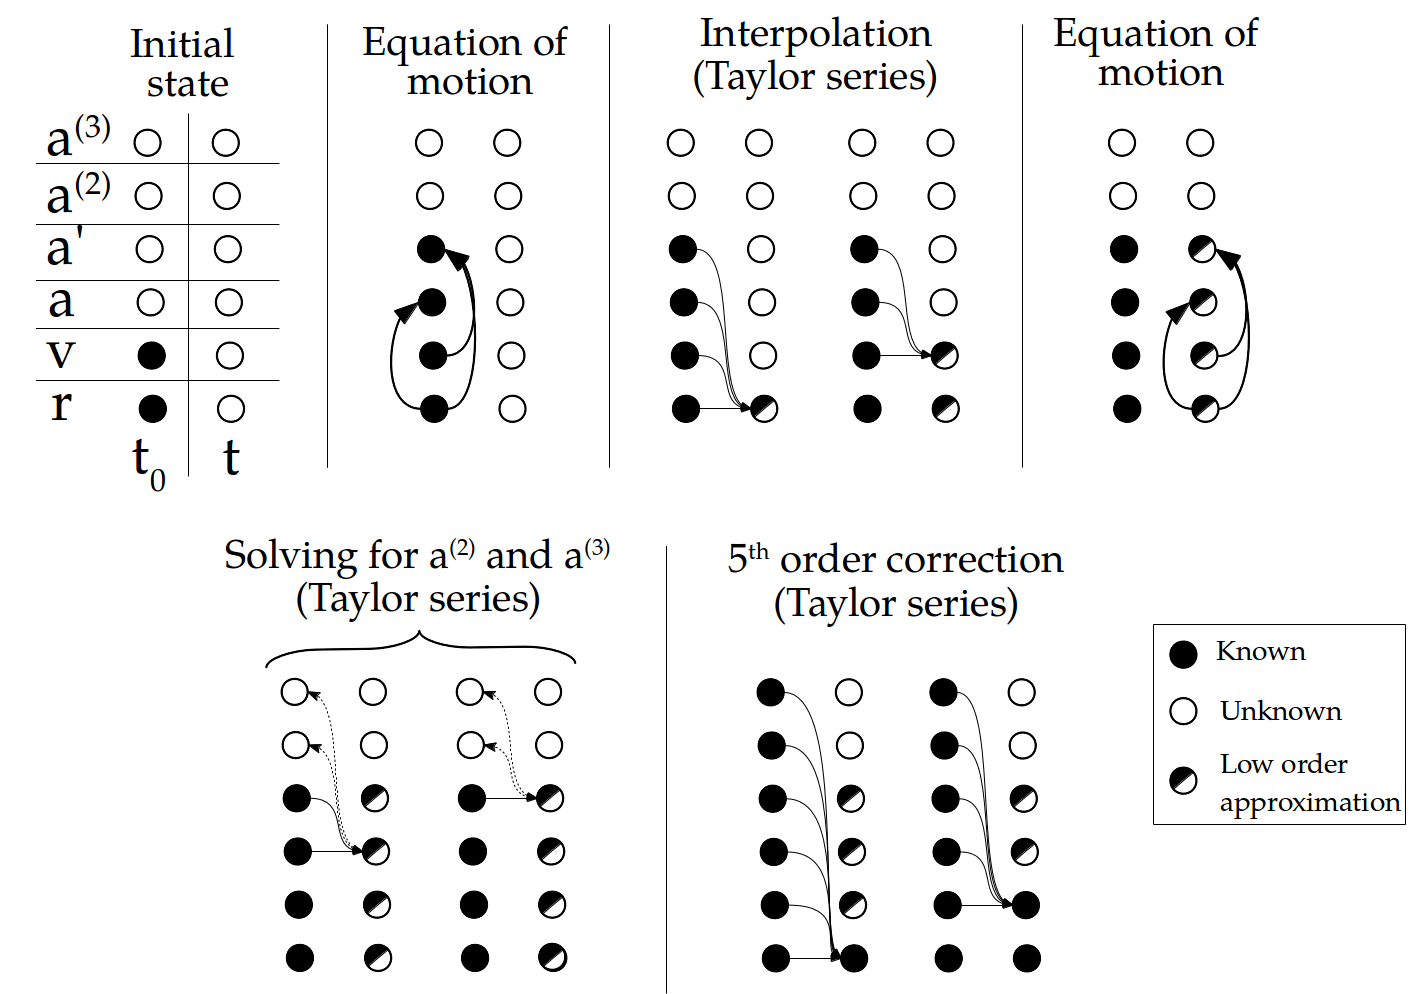
\includegraphics[width=0.9\linewidth]{Figures/0_hermite_scheme.png}
\caption{Summary of the Hermite scheme starting from known positions and velocities at $t_0$ to obtain 5th order values at t.}
\label{Fig:0_hermite_scheme}
\end{figure} 
 

\begin{align}
\label{Eq:0_Hermite_acc1}
\bold{a}_{0,i} &= - \sum\limits_{i\neq j} G m_j \frac{\bold{R}}{R^3}\\
\label{Eq:0_Hermite_acc2}
\dot{\bold{a}}_{0,i} &=  - \sum\limits_{i\neq j} G m_j \left[ \frac{\bold{V}}{R^3}  + 
	\frac{ 3 \bold{R} ( \bold{V} \cdot \bold{R} )  }{R^3}\right]
\end{align}
with $\bold{R} = \bold{r}_{0,i} - \bold{r}_{0,j} $ and $\bold{V} = \bold{v}_{0,i} - \bold{v}_{0,j} $. Using these quantities, it is now possible to predict the positions and velocities at $t$ through a Taylor serie, again for all particles $i$:

\begin{align}
\bold{r}_{p,i}(t) &= \bold{r}_0 + \bold{v}_0 (t-t_0) + \bold{a}_{0,i}\frac{(t-t_0)^2}{2!} 	
		 +\dot{\bold{a}}_{0,i}\frac{(t-t_0)^3}{3!}\\
\bold{v}_{p,i}(t) &= \bold{v}_0 + \bold{a}_{0,i}(t-t_0) + \dot{\bold{a}}_{0,i}\frac{(t-t_0)^2}{2!}
\end{align}.

The predicted accelerations and their derivatives $\bold{a}_{p,i}(t)$,  $\dot{\bold{a}}_{p,i}(t)$ are computed by injecting $\bold{r}_{p,i}(t)$ and $\bold{v}_{p,i}(t)$ into equations \ref{Eq:0_Hermite_acc1} and \ref{Eq:0_Hermite_acc2}. The accelerations at t, of which predicted values have just been computed, can also be obtained through Taylor series:

\begin{align}
\label{Eq:0_Hermite_taylor1}
\bold{a}_{i}(t) &= \bold{a}_{0,i} + \dot{\bold{a}}_{0,i} (t-t_0) + \bold{a}^{(2)}_{0,i}\frac{(t-t_0)^2}{2!} + \bold{a}^{(3)}_{0,i}\frac{(t-t_0)^3}{3!}\\
\label{Eq:0_Hermite_taylor2}
\dot{\bold{a}}_{i}(t) &=  \dot{\bold{a}}_{0,i} +  \bold{a}^{(2)}_{0,i}(t-t_0) + \bold{a}^{(3)}_{0,i}\frac{(t-t_0)^2}{2!}
\end{align}
with $\bold{a}^{(2)}_{0,i}$,$\bold{a}^{(3)}_{0,i}$ the third and fourth derivative of the acceleration at $t=0$. Note that these quantities are unknown for now. To take the derivatives of equation \ref{Eq:0_Hermite_acc2} would be too computationnaly expansive. Instead, $\bold{a}_{p,i}(t)$ and  $\dot{\bold{a}}_{p,i}(t)$ are injected in the left hand side of equations \ref{Eq:0_Hermite_taylor1} and \ref{Eq:0_Hermite_taylor2} and solved for $\bold{a}^{(2)}_{0,i}$ and $\bold{a}^{(3)}_{0,i}$. This leads to the expressions:

\begin{align}
\bold{a}^{(3)}_{0,i} &= 12 \frac{\bold{a}_{0,i} - \bold{a}_{p,i}}{(t-t_0)^3} +6 \frac{\dot{\bold{a}}_{0,i} - \dot{\bold{a}}_{p,i}}{(t-t_0)^3}\\
\bold{a}^{(2)}_{0,i} &= -6 \frac{\bold{a}_{0,i} - \bold{a}_{p,i}}{(t-t_0)^2} - 2 \frac{2\dot{\bold{a}}_{0,i} + \dot{\bold{a}}_{p,i}}{t-t_0}.
\end{align}

The predicted values of positions and velocities are then corrected using the second and third order derivatives of acceleration, yeilding fifth order accurate values.

\begin{align}
\bold{r}_{c,i}(t) &= \bold{r}_{p,i}(t) + \bold{a}^{(2)}_{0,i} \frac{(t-t_0)^4}{4!} +
	 \bold{a}^{(3)}_{0,i} \frac{(t-t_0)^5}{5!}\\
\bold{v}_{c,i}(t) &= \bold{v}_{p,i}(t) + \bold{a}^{(2)}_{0,i} \frac{(t-t_0)^3}{3!} +
	 \bold{a}^{(3)}_{0,i} \frac{(t-t_0)^4}{4!}\\
\end{align}



In a nutshell, the Hermite scheme is a way to obtain 5th order terms with limited cost. The steps are summarised in figure \ref{Fig:0_hermite_scheme}. First $r_0^{(2)}$ and $r_0^{(3)}$ are computed, then used to obtain predictions of $r_t^{(0)}$ and $r_t^{(1)}$, transformed with the equations of motions into predictions of $r_t^{(3)}$ and $r_t^{(4)}$. These last two can be expressed through Taylor series as functions of $r_0^{(3)}$,$r_0^{(4)}$ and $r_0^{(5)}$, which are solved for these last two terms. The predicted values of $r_t^{(0)}$ and $r_t^{(1)}$ are then corrected to the fifth order with $r_0^{(4)}$ and $r_0^{(5)}$.

The error for a single time step scales as $O(\Delta t^5)$. The Hermite scheme has shown itself very well suited for the block time step method, as the synchronization of particles limit the amount of prediction to be made, many positions at a given time being already known and computed with maximum accuracy.


\subsection{Ahmad-Cohen neighbour scheme}

For a given particle in an nbody system, the influence of direct neighbours changes on shorter timescales than the smooth potential from distant particles. The essence of the Ahmad-Cohen neighbour scheme is to decouple the two for computational efficiency \citep{AhmadCohen1973}. The acceleration is splitted into two components:

\begin{equation}
\bold{a}_i = \bold{a}_{i,reg} + \bold{a}_{i,irr}
\end{equation}

$\bold{a}_{i,irr}$ is the acceleration from particles inside a given "neighbour sphere" around particle $i$, while $\bold{a}_{i,reg}$ is the acceleration from all other, more distant, particles. Integration within the neighbours sphere,  \textit{irregular} integration, is decoupled from the global, \textit{regular}, integration. Regular time steps, where complete force summation are performed over all particles with eq \ref{Eq:0_Hermite_acc1}, are subdivided into irregular time steps, where regular acceleration is predicted and irregular acceleration is computed through a force summation on the $N_{i,nb}$ neighbours. The list of neighbours of $i$ is updated every regular time step and contains the particles within a sphere of radius $R_{i,s}$ centered on $i$. Are also added to the neighbour list are the particles within $2^{\frac{1}{3}}R_{i,s} $ that satisfy the condition
\begin{equation}
\bold{R} \cdot \bold{V} < 0.1 \frac{R_s^2}{\Delta T_{reg}}
\end{equation}
with $\Delta T_{reg}$ the regular time step. This ensures that fast approaching particles are selected before they enter the actual neighbour sphere. $R_{i,s}$ is determined through local number density contrast and optimisation of the resulting $N_{i,nb}$. 

When $N_{nb} \ll N$ for most particles, there is a great performance improvement, without loss of accuracy. 












